
% \chapter{Analytical Techniques and Tools}
% \label{chap:tech-tools}
% \begin{small}
% \begin{quote}
%   \emph{``Any engineer or computer scientist who has designed,
%     certified, or worked with systems of any size or consequence knows
%     that a key question is \emph{how will we know?} $\ldots$ They know
%     that undetected flaws potentially destroy systems, destroy
%     reputations, and destroy credibility, leading to failed missions,
%     failed services, and failed corporations. In short, as systems
%     become larger and more complex, it is increasingly difficult for
%     designers to get a good night's sleep.''}
% \end{quote}
% \hfill{Shiu-Kai Chin and Sue Older, \emph{Access Control, Security,
%     and Trust: A Logical Approach}}

% \begin{quote}
%     \emph{``I want theorems!''}
% \end{quote}
% \hfill{Dr. Kamal Jabbour, ST, Senior Scientist for Information
%   Assurance, AFRL }
  
% \end{small}


% \section{Introduction}
% \label{sec:introduction}

% Our analysis and solutions rely on the following:
% \begin{enumerate}
% \item an \emph{access-control logic} used to describe and verify
%   access-control policies and decisions,
% \item \emph{structural operational semantics} to specify and verify
%   our expectations of outcomes of computations, and
% \item the Higher Order Logic (HOL) proof checker for formally verifying
%   the correctness of our analysis and solutions.
% \end{enumerate}
% Overviews of these techniques and tools are described in
% Sections~\ref{sec:access-control-logic}, \ref{sec:struct-oper-semant},
% and \ref{sec:higher-order-logic}, respectively. 

\chapter{Access-Control Logic: Syntax and Semantics}
\label{cha:access-control-logic}

The access-control logic we use is fully described in \emph{Access
  Control, Security, and Trust: A Logical Approach}, \cite{ACST}. It
is a multi-agent modal logic with Kripke semantics.  We present an
overview of the logic consisting of its syntax, semantics, and
inference rules. This presentation is almost identical with our
overview of the logic in \cite{DBLP:conf/mmmacns/ChinMOV10}.

\section{Syntax}
\label{sec:syntax}

\paragraph{Principal Expressions}

Let $P$ and $Q$ range over a collection of principal expressions. Let
$A$ range over a countable set of simple principal names. The abstract
syntax of principal expressions is:
\begin{align*}
P ::= A \ora P \with Q \ora P\quoting Q 
\end{align*}
The principal $P \with Q$ (``$P$ in conjunction with $Q$'') is an
abstract principal making exactly those statements made by both $P$
and $Q$; $P\quoting Q$ (``$P$ quoting $Q$'') is an abstract
principal corresponding to principal $P$ quoting principal $Q$.

\paragraph{Access Control Statements}

The abstract syntax of statements (ranged over by $\varphi$) is
defined as follows, where $P$ and $Q$ range over principal expressions
and $p$ ranges over a countable set of
\emph{propositional variables}:
\begin{eqnarray*}
  \varphi &::=&  p \ora  \neg \varphi 
  \ora  \varphi_1 \wedge \varphi_2
  \ora  \varphi_1 \vee \varphi_2
  \ora  \varphi_1 \implies \varphi_2 \ora \varphi_1 \equiv \varphi_2 \ora\\
  & &  P \speaksfor Q 
  \ora P \says \varphi 
  \ora P \controls \varphi
  \ora \reps{P}{Q}{\varphi}
\end{eqnarray*}

Informally, a formula $P \speaksfor Q$ (pronounced ``$P$ speaks for
$Q$'') indicates that \emph{every} statement made by $P$ can also be
viewed as a statement from $Q$.  A formula $P \controls \varphi$ is an
abbreviation for the implication $(P \says \varphi) \implies \varphi$:
in effect, $P$ is a trusted authority with respect to the statement
$\varphi$. $\reps{P}{Q}{\varphi}$ denotes that $P$ is $Q$'s delegate
on $\varphi$; it is an abbreviation for $(P \says (Q \says \varphi))
\implies Q \says \varphi$. Notice that the definition of
$\reps{P}{Q}{\varphi}$ is a special case of $\controls$ and in effect
asserts that $P$ is a trusted authority with respect to $Q$ saying
$\varphi$.

\section{Semantics}
\label{sec:semantics}


Kripke structures define the semantics of formulas.


\begin{definition}
    A \emph{Kripke structure} $\mathcal{M}$ is a three-tuple
  $\krip{W,I,J}$, where:
  \begin{itemize}
  \item $W$ is a nonempty set, whose elements are called \emph{worlds}. 
    
  \item $I: \PropVar \arrow \pow{W}$ is an \emph{interpretation}
    function that maps each propositional variable $p$ to a set of
    worlds.

  \item $J: \PName \arrow \pow{W\times W}$ is a function that maps each
    principal name $A$ to a relation on worlds (i.e., a subset of
    $W\times W$).
  \end{itemize}
 
\end{definition}

% Just as the interpretation function $I$ of a Kripke structure provides
% the base interpretation for propositional variables, the function $J$
% provides a base interpretation for simple principal names.  
We extend $J$ to work over arbitrary \emph{principal expressions}
using set union and relational composition. The extended function
$\hat{J}$ is defined as follows:
\begin{eqnarray*}
  \hat{J}(A) & = & J, \text{ where $A$ is a simple principal name}\\
  \hat{J}(P \with Q) & = & \hat{J}(P) \cup \hat{J}(Q) \\
  \hat{J}(P \quoting Q) & = & \hat{J}(P) \circ \hat{J}(Q),  
\end{eqnarray*}
where
\begin{gather*}
  \hat{J}(P) \circ \hat{J}(Q) = \{(w_1, w_2) \mid \exists w'. (w_1,
  w') \in \hat{J}(P) \text{ and } (w', w_2) \in \hat{J}(Q)\}
\end{gather*}
\begin{definition}
  Each Kripke structure $\mathcal{M} = \krip{W,I,J}$ gives rise to a
  function 
  \[ \E{-}: \LExp \arrow \pow{W}, \]
  where $\E{\varphi}$ is the set of worlds in which $\varphi$ is
  considered true.
%
  \E{\varphi} is defined inductively on the structure of $\varphi$, as
  shown in Figure~\ref{fig:semantics}.

  \begin{figure}[tb]
    \centering
    \begin{minipage}[h]{0.7\linewidth}
    \begin{center}
    \begin{small}
    \begin{align*}
      \E{p}       & = I(p)\\
      \E{\neg \varphi} & = W - \E{\varphi}\\
      \E{\varphi_1 \wedge \varphi_2} & = \E{\varphi_1} \cap
      \E{\varphi_2}\\
      \E{\varphi_1 \vee \varphi_2} & = \E{\varphi_1} \cup \E{\varphi_2}\\
      \E{\varphi_1 \implies \varphi_2} & = (W - \E{\varphi_1}) \cup
      \E{\varphi_2} \\
      \E{\varphi_1 \equiv \varphi_2} & = \E{\varphi_1 \implies
        \varphi_2} \cap \E{\varphi_2 \implies \varphi_1} \\
%      & & \\
      \E{P \speaksfor Q} &= 
      \begin{cases}
        W, & \text{if $J(Q) \subseteq J(P)$} \\
        \emptyset, & \text{otherwise}
      \end{cases} \\
      \E{P \says \varphi} & = \{w | J(P)(w) \subseteq \E{\varphi}\} \\
      \E{P \controls \varphi} & = \E{(P \says \varphi) \implies \varphi}
      \\
      \E{\reps{P}{Q}{\varphi}} & = \E{P \quoting Q \says \varphi \implies Q
        \says \varphi}
    \end{align*}\vspace*{-0.3in}
    \end{small}
    \end{center}
    \end{minipage}

    \caption{Semantics}
    \label{fig:semantics}
  \end{figure}

Note that, in the definition of \E{P \says \varphi}, $J(P)(w)$ is simply
the image of world $w$ under the relation $J(P)$.
\end{definition}


\section{Inference Rules}
\label{sec:inference rules}

In practice, relying on the Kripke semantics alone to reason about
policies, concepts of operations (CONOPS), and behavior is
inconvenient. Instead, inference rules are used to manipulate formulas
in the logic. All logical rules must be sound to maintain consistency.

\begin{definition}
  A rule of form $\irule{H_1 \cdots H_n}{C}{}$ is sound if,
  \textsl{for all Kripke structures $\mathcal{M} = \langle W, I, J
    \rangle$, if $\E{H_i}=W$ for each $i \in \{1,\ldots, n\}$, then
    $\E{C} = W$}.
\end{definition}

The rules in Figures~\ref{fig:inference-rules}
and~\ref{fig:derived-rules} are all sound. As an additional check, the
logic and rules have been implemented in the HOL-4 (Higher Order
Logic) theorem prover as a conservative extension of the HOL logic
\cite{HOL}.


% The Kripke structures are then only necessary if one wishes to add
% new inference rules and to verify their soundness.  The semantic
% functions $\mathcal{E}_{\mathcal{M}}$ provide a fully defined and
% fully disclosed interpretation for the formulas of the logic.  This
% mathematical foundation enables us to provide a means to reason
% about access-control situations using a small core collection of
% sound inference rules and syntactic-sugar definitions (see
% Figure~\ref{fig:inference-rules}), along with a larger set of rules
% that can be formally derived from the core rules (see
% Figure~\ref{fig:derived-rules} for a sample set of derived rules
% that we have found particularly useful).


% (In proofs, if we have the terms $H_1$ through $H_n$ we can infer $C$ and
% know the inference is sound.)  

  \begin{figure}[tb]
    \centering
    \begin{footnotesize}

    \irule{}{\qquad\varphi\qquad}{Taut} $\quad$ \parbox{1.4in}{if
      $\varphi$ is an  
      instance of a prop-logic tautology}    \rulespace

    \irule{\varphi \qquad  \varphi \implies \varphi'}{\varphi'}{Modus\
      Ponens}
    \hspace*{3em}
    \irule{\varphi}{P \says \varphi}{Says}
    \rulespace
    
    \irule{}{(P \says (\varphi \implies \varphi')) \implies (P \says
      \varphi \implies P \says \varphi')}{MP\ Says} \rulespace
    
    \irule{}{P \speaksfor Q \implies (P \says \varphi \implies Q \says
      \varphi)}{Speaks For} 
    \rulespace

    \irule{}{P \quoting Q \says \varphi \equiv P \says  Q \says
      \varphi}{Quoting}\rulespace 

    \irule{}{P \with Q \says \varphi \equiv P \says \varphi \wedge  Q \says
      \varphi}{$\with$Says}\rulespace 

    \irule{}{P \speaksfor P}{Idempotency of $\speaksfor$} \qquad
    \irule{P' \speaksfor P \quad Q' \speaksfor Q}{P' \quoting Q'
      \speaksfor P \quoting Q}{Monotonicity of $\quoting$} \vspace*{2ex}

    \irule{P \quoting (Q \quoting R) \says \varphi}{ (P \quoting Q) \quoting
      R \says \varphi}{Associativity of $\quoting$}\rulespace

    $P \controls \varphi \quad \defn \quad (P \says \varphi) \implies
    \varphi$ \vspace*{2ex}

    $\reps{P}{Q}{\varphi} \defn P \quoting Q \says \varphi\implies Q
    \says \varphi$ 
    \end{footnotesize}
    \caption{Core Inference Rules}
    \label{fig:inference-rules}
  \end{figure}

  \begin{figure}[t]
    \centering
    \begin{footnotesize}
%     \irule{\varphi_1 \qquad \varphi_2}{\varphi_1 \wedge
%       \varphi_2}{Conjunction} 
%     \rulespace
%    \irule{\neg \neg \varphi}{\varphi}{Double\ negation}
%    \rulespace


%     \irule{\varphi_1 \wedge \varphi_2}{\varphi_1}{Simplification (1)} 
%     \hspace*{2em}
%     \irule{\varphi_1 \wedge \varphi_2}{\varphi_2}{Simplification (2)} 
%     \rulespace

%    \irule{\varphi_1}{\varphi_1 \vee \varphi_2}{Disjunction} 
%    \hspace*{2em}
%    \irule{\varphi_2}{\varphi_1 \vee \varphi_2}{Disjunction} 
%    \rulespace
   
%    \irule{\varphi \implies \varphi' \quad \neg \varphi'}{\neg
%      \varphi}{\parbox{.5in}{Modus \\ Tollens}}
%%    \hspace*{2em}
%    \rulespace

%    \irule{\varphi_1 \implies \varphi_2 \quad \varphi_2 \implies
%      \varphi_3}{\varphi_1 \implies
%      \varphi_3}{\parbox{.65in}{Hypothetical \\ Syllogism}} 
%    \rulespace

%    \irule{\varphi_1 \vee \varphi_2 \quad \neg
%      \varphi_1}{\varphi_2}{\parbox{.6in}{Disjunctive \\ Syllogism}}
%%    \hspace*{2em}
%    \rulespace
%      \irule{\varphi_1 \equiv \varphi_2 \quad
%        \varphi_1}{\varphi_2}{$Equiv_1$} \qquad
%      \irule{\varphi_1 \equiv \varphi_2 \quad
%        \varphi_2}{\varphi_1}{$Equiv_2$} \rulespace

    \irule{P \quoting Q \says \varphi}{P \says Q \says \varphi}{Quoting
      (1)} \qquad
    \irule{P \says Q \says \varphi}{P \quoting Q \says \varphi}{Quoting
      (2)} \rulespace

%     \irule{P\with Q \says \varphi}{P \says \varphi \wedge Q \says
%       \varphi}{$\with$Says (1)} \qquad
%     \irule{P \says \varphi \wedge Q \says\varphi}{P\with Q \says
%       \varphi}{$\with$Says (2)} \rulespace

    \irule{P \controls \varphi \quad P \says \varphi}{\varphi}{Controls}
    \qquad
    \irule{P \speaksfor Q \quad P \says \varphi}{Q \says
      \varphi}{Derived Speaks For}
    \rulespace

    \irule{Q \controls \varphi \quad \reps{P}{Q}{\varphi} \quad
      P\quoting Q \says \varphi}{\varphi}{Reps} \rulespace

    \irule{\reps{P}{Q}{\varphi} \quad P \quoting Q \says \varphi}{Q
      \says \varphi}{Rep Says}

    \end{footnotesize}
    \caption{Derived Rules Used in this Report}
    \label{fig:derived-rules}
  \end{figure}

\section{Confidentiality and Integrity Policies}

Confidentiality and integrity policies such as Bell-LaPadula
\cite{BL73} and Biba's Strict Integrity policy \cite{Biba77}, depend
on classifying, i.e., assigning a confidentiality or integrity level
to information, subjects, and objects. It is straightforward to extend
the access-control logic to include confidentiality, integrity, or
availability levels as needed. In what follows, we show how the syntax
and semantics of \emph{integrity} levels are added to the core
access-control logic. The same process is used for levels used for
\emph{confidentiality} and \emph{availability}.

\paragraph{Syntax}

The first step is to introduce syntax for describing and comparing
security levels. \IntLabelConst is the collection of \emph{simple
  integrity labels}, which are used as names for the integrity
levels (e.g., \textsc{hi} and \textsc{lo}).

Often, we refer abstractly to a principal $P$'s integrity level.  We
define the larger set \IntLevel of \emph{all} possible integrity-level
expressions:
\begin{eqnarray*}
  \IntLevel &\isa& \IntLabelConst \ora  \ilv{\PName}.
\end{eqnarray*}
An integrity-level expression is either a simple integrity label or an
expression of the form $\ilv{A}$, where $A$ is a \emph{simple
  principal name}.  Informally, $\ilv{A}$ refers to the integrity
level of a simple principal $A$. Note, we do not define (and leave
unspecified) the definition of mapping of \emph{compound} principal
expressions to labels.

Finally, we extend our definition of well-formed formulas to support
comparisons of integrity levels:
\begin{eqnarray*}
    \LExp &::=&  \IntLevel \leq_i \IntLevel \ora \IntLevel =_i \IntLevel 
\end{eqnarray*}
Informally, a formula such as $\textsc{lo} \leq_i \ilv{\name{Kate}}$
states that Kate's integrity level is greater than or equal to (i.e.,
\emph{dominates}) the integrity level \textsc{lo}.  Similarly, a
formula such as $\ilv{\name{Barry}} =_i \ilv{\name{Joe}}$ states that
Barry and Joe have the same integrity level.

\paragraph*{Semantics}

Providing formal and precise meanings for the newly added syntax
requires us to extend our Kripke structures with additional components
that describe integrity classification levels.  Specifically, we
introduce extended Kripke structures of the form
\[ \mathcal{M} = \krip{W,I,J,K,L,\preceq}, \]
where:
\begin{itemize}
\item $W$, $I$, and $J$ are as defined earlier.
\item $K$ is a non-empty set, which serves as the universe of 
  \emph{integrity levels}.
\item $L: (\IntLabelConst \cup \PName) \arrow K$ is a function that maps
  each integrity label and each simple principal name to a integrity
  level. $L$ is extended to work over arbitrary integrity-level
  expressions, as follows:
  \[ L(\ilv{A}) = L(A), \]
  for every simple principal name $A$.
\item $\preceq \subseteq K\times K$ is a partial order on $K$: that is,
  $\preceq$ is \emph{reflexive} (for all $k\in K$, $k \preceq k$),
  \emph{transitive} (for all $k_1,k_2,k_3\in K$, if $k_1 \preceq k_2$
  and $k_2 \preceq k_3$, then $k_1 \preceq k_3$), and
  \emph{anti-symmetric} (for all $k_1,k_2\in K$, if $k_1 \preceq
  k_2$ and $k_2\preceq k_1$, then $k_1 = k_2$).
\end{itemize}

Using these extended Kripke structures, we extend the semantics for
our new well-formed expressions as follows:
\begin{eqnarray*}
   \E{\ell_1 \leq_i \ell_2} &=&
   \begin{cases}
     W, & \text{ if } L(\ell_1) \preceq L(\ell_2) \\
     \emptyset, & \text{otherwise} 
   \end{cases} \\
   \E{\ell_1 =_i \ell_2} &=& \E{\ell_1 \leq_i \ell_2} \cap \E{\ell_2
     \leq_i \ell_1}.
\end{eqnarray*}
As these definitions suggest, the expression $\ell_1 =_i \ell_2$ is
simply an abbreviation for $(\ell_1 \leq_i \ell_2) \wedge (\ell_2
\leq_i \ell_1)$.

\paragraph*{Logical Rules}

Based on the extended Kripke semantics we introduce logical rules that
support the use of integrity levels to reason about access requests.
Specifically, the definition, reflexivity, and transitivity rules in
Figure~\ref{fig:integrity-level-rules} reflect that $\leq_i$ is a
partial order. The fourth rule is derived and convenient to have.

\begin{figure}[t]
  \centering
\begin{small}
  $\ell_1 =_i \ell_2 \defn (\ell_1 \leq_i \ell_2) \wedge (\ell_2 \leq_i
  \ell_1)$ \vspace*{1em} 
  
  \irule{}{\ell \leq_i \ell}{Reflexivity of $\leq_i$} \vspace*{1em} 

  \irule{\ell_1 \leq_i \ell_2 \qquad \ell_2 \leq_i \ell_3}{\ell_1 \leq_i
    \ell_3}{Transitivity of $\leq_i$}  \vspace*{1em}

  \irule{\ilv{P} =_i \ell_1 \quad \ilv{Q} =_i \ell_i \quad \ell_1 \leq_i
    \ell_2}{\ilv{P} \leq_i \ilv{Q}}{sl $\leq_i$} 
\end{small}
  \caption{Inference rules for relating integrity levels}
  \label{fig:integrity-level-rules}
\end{figure}

\section{Examples}
\label{sec:examples}

The following two examples in Sections~\ref{sec:simple-example} and
\ref{sec:an-integrity-example} illustrate the use of the core
inference rules to derive new inference rules. The first example
proves the \emph{Controls} rule. The second example is a more involved
example illustrating the use of partial orders on integrity labels to
make access-control decisions.

\subsection{A simple example}
\label{sec:simple-example}

We prove the \emph{Controls} rule in Figure~\ref{fig:derived-rules}
using the core inference rules in
Figure~\ref{fig:inference-rules}. The proof is simple and is shown in
Figure~\ref{fig:controls-proof}.  The first two lines are the
assumptions of the \emph{Controls} rule. The third and fourth lines
are derived as applications the core inference rules \emph{Definition
  of Controls} and \emph{Modus Ponens}.

\begin{figure}[t]
  \centering
  \begin{tabular}{r<{.} >{$}p{0.3\linewidth}<{$}p{0.3\linewidth}}
    1 & P \controls \varphi & assumption\\
    2 & P \says \varphi & assumption\\
    3 & (P \says \varphi) \implies \varphi & 1 Definition of Controls\\
    4 & \varphi & 2, 3 Modus Ponens
  \end{tabular}
  
  \caption{Proof of Controls Inference Rule}
\label{fig:controls-proof}
\end{figure}


\subsection{An Integrity Example}
\label{sec:an-integrity-example}

This a simple example of Biba's Strict Integrity model,
\cite{Biba77}. In this model a subject $S$ can only read or take from
an object $O$ if the object's integrity level is at least as high or
greater than $S$'s. Similarly, subject $S$ can only write or modify
$O$ if $S$'s integrity level is at least as high or greater than
$O$'s. This policy prevents contamination or corruption of subjects
and objects from the standpoint of quality or integrity.

\begin{figure}[t]
  \centering
  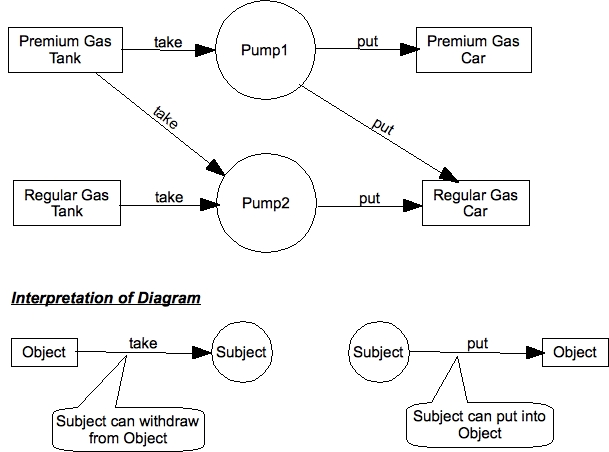
\includegraphics[width=0.6\linewidth]{Figures/gasSolution}  
  \caption{Access Diagram for Gas}
  \label{fig:access-diagram}
\end{figure}

Consider the following scenario. There are two grades of gas: \emph{P}
for premium gas and \emph{R} for regular gas.  There are two pumps:
\emph{Pump1} and \emph{Pump2}. There are two cars: a car that uses regular
gas (\emph{RGC}) and a car that requires premium gas (\emph{PGC}).

We assume the typical relation on gas grades: premium gas is higher
quality than regular gas, i.e., $R \leq_i P$. We also assume cars
specified as taking a particular grade of gas can safely take that
grade of gas or higher. In our example, \emph{RGC} can be fueled with
regular (R) gas or premium (P) gas, whereas \emph{PGC} can only be
fueled with premium (P) gas.

Figure~\ref{fig:access-diagram} diagrams the subjects, objects, and
types of access permitted in this scenario. Informally, subjects
\emph{act} on objects. The subjects in the scenario are \emph{Pump1}
and \emph{Pump2}.  The objects are the Premium Gas Tank \emph{(PGT)},
the Regular Gas Tank \emph{(RGT)}, the Premium Gas Car \emph{(PGC)}, and
the Regular Gas Car \emph{(RGC)}. What the diagram shows is that
\emph{Pump1} can only take or pump premium gas.  It can put gas into
both the regular and premium gas cars.  \emph{Pump2} can take or draw
from both premium and regular gas tanks, but it can only put gas into
the regular gas car.

\begin{table}[t]
  \centering
\begin{tabular}[h]{r | c}
  \emph{Subjects and Objects} & \emph{Integrity Level}\\
  \hline
  Premium Gas Tank \emph{PGT} & P\\
  Regular Gas Tank \emph{RGT} & R\\
  Pump1  & P\\
  Pump2& R\\
  Premium Gas Car \emph{PGC} & P\\
  Regular Gas Car \emph{RGC} &R\\
\end{tabular}
  \caption{Integrity Level Assignments}
  \label{tab:int-level-assignments}
\end{table}

\begin{table}[t]
  \centering
  \begin{tabular}[h]{r | c c c c}
    \textbf{Subject} & \textbf{PGT (P)} & \textbf{RGT (R)} &
    \textbf{PGC (P)} &
    \textbf{RGC (R)}\\
    \hline
    \emph{Pump1 (P)} & take & - & put & put\\
    \emph{Pump2 (R)} & take & take & - & put\\
  \end{tabular}
  \caption{Access-Control Matrix}
  \label{tab:access-control-matrix}
\end{table}

If we use $P$ as the integrity level for premium grade and $R$ as the
integrity level for regular grade, the subjects and objects have the
integrity level assignments shown in
Table~\ref{tab:int-level-assignments}. These assignments combined with
the access privileges shown in Figure~\ref{fig:access-diagram} result
in the access-control matrix in
Table~\ref{tab:access-control-matrix}.

Under the assumption that the integrity levels are \emph{partially
  ordered}, i.e., $R \leq_i R$, $P \leq_i P$, and $R \leq_i P$, we see
that the assignment of access rights in
Table~\ref{tab:access-control-matrix} conforms with Biba's Strict
Integrity policy. No car, in this assignment of \emph{take} and
\emph{put} privileges, can be filled with gas of lesser quality than
it is specified to take.

Using the access-control logic, we can formally represent the
access-control policy as shown in Figure~\ref{fig:access-control-gas},
where each formula describes the conditions under which it is
permitted for Pump1 or Pump2 to exercise a take or put privilege on an
object.
\begin{figure}[t]
  \centering
  \begin{align*}
    \ilv{Pump1} \leq_i \ilv{PGT} &\implies Pump1 \controls \action{take,PGT}\\
    \ilv{PGC} \leq_i \ilv{Pump1} &\implies Pump1 \controls \action{put,PGC}\\
    \ilv{RGC} \leq_i \ilv{Pump1} &\implies Pump1 \controls \action{put,RGC}\\
    \ilv{Pump2} \leq_i \ilv{PGT} &\implies Pump2 \controls \action{take,PGT}\\
    \ilv{Pump2} \leq_i \ilv{RGT} &\implies Pump2 \controls \action{take,RGT}\\
    \ilv{RGC} \leq_i \ilv{Pump2} &\implies Pump2 \controls
    \action{put,RGC}
  \end{align*}
  
  \caption{Access-Control Policy for Pumping Gas}
\label{fig:access-control-gas}
\end{figure}



\begin{figure}[t]
  \centering
\begin{tabular}{r<{.} >{$}p{0.7\linewidth}<{$}p{0.3\linewidth}}
  1 & Pump1 \says \action{put,PGC} & request\\
  2 & \ilv{PGC} \leq_i \ilv{Pump1} \implies Pump1 \controls \action{put,
        PGC}& integrity policy\\
  3 & \ilv{PGC} =_i P & level assignment\\
  4 & \ilv{Pump1} =_i P& level assignment\\
  5 & \ilv{P} \leq_i \ilv{P} & Reflexivity of $\leq_i$\\
  6 & \ilv{PGC} \leq_i \ilv{Pump1} & 3, 4, 5 $\leq_i$ Subst\\
  7 & Pump1 \controls \action{put, PGC} & 2, 6 Modus Ponens\\
  8 &  \action{put, PGC} & 7, 1 Controls
\end{tabular}  
  \caption{Pump1 Proof}
  \label{fig:pump1-proof}
\end{figure}

As an illustration, consider a request by \emph{Pump1} to put gas into
the premium-gas car \emph{PGC}. This request is formally represented as
\begin{gather*}
  Pump1 \says \action{put, PGC}.
\end{gather*}
We wish to determine if we should honor the request, i.e., if we can
conclude $\action{put, PGC}$. The relevant access-policy statement
from Table~\ref{tab:access-control-matrix} is
\begin{gather*}
  \ilv{PGC} \leq_i \ilv{Pump1} \implies Pump1 \controls \action{put,
    PGC}.
\end{gather*}
From Table~\ref{tab:int-level-assignments} we get the integrity level
assignments of \emph{Pump1} and \emph{PGC}:
\begin{gather*}
  \ilv{PGC} =_i P \text{ and } \ilv{Pump1} =_i P.
\end{gather*}
The request with the policy and level assignment statements is enough
to prove a theorem or derived inference rule justifying letting
\emph{Pump1} put gas into \emph{PGC}.  The derived inference rule is
below. Its proof is shown in Figure~\ref{fig:pump1-proof}.
\begin{gather*}
  \irule
  {
    \begin{array}{c}
      Pump1 \says \action{put, PGC}\\
      \ilv{PGC} \leq_i \ilv{Pump1} \implies Pump1 \controls \action{put,
        PGC}\\
      \ilv{PGC} =_i P \qquad \ilv{Pump1} =_i P
    \end{array}
  } 
  {\action{put, PGC}} 
  {}.
\end{gather*}


% \chinbox{
%   \begin{itemize}
%   \item Pump1 request to put gas into PGC
%   \item Derived theorem/inference rule justifying request
%   \item Refer to proof in Figure~\ref{fig:pump1-proof}
%   \end{itemize}
% }

% \section{Structural Operational Semantics}
% \label{sec:struct-oper-semant}

% Structural operational semantics (SOS) deals with the \emph{behavior}
% of programs, \cite{Plotkin04} and \cite{Huttel10}. It uses mathematics
% to describe and reason about the behavior of programs. We will use SOS
% to describe and reason about the expected behavior of cloud services
% and hardware devices.

% Structural operational semantics is defined in terms of the
% \emph{syntax} or \emph{structure} of a language or program. The
% underlying behavioral definitions use mathematical \emph{induction} to
% relate values to programs or language expressions.

% As a tutorial example, we develop the structural operational semantics
% for a simple arithmetic expression language, \textbf{AExp}. First, we
% introduce the syntax of \textbf{AExp}. Second, we define the semantics
% of \textbf{AExp}.

% \subsection{Syntax of AExp}
% \label{sec:syntax-aexp}

% Our illustrative example is to define the structural operational
% semantics for simple arithmetic expressions described by the set of
% formulas \textbf{AExp}. \textbf{AExp} is built on the set of natural
% numbers, which we call \textbf{num}.
% \begin{align*}
%   num &= \set{0, 1, 2, 3, \cdots}\\
%   AExp &::= const\;num \ora plus \;AExp_1\; AExp_2 \ora minus\; AExp_1
%   \;AExp_2 \ora times \;AExp_1\; AExp_2
% \end{align*}

% From the abstract syntax rule for \textbf{AExp} formulas above, we see
% that AExp expressions have one of four forms. Arithmetic expressions
% as defined are either:
% \begin{enumerate}
% \item a constant, i.e., \emph{const} followed by a natural number
%   (\emph{num}),
% \item \emph{plus} followed by two AExp expressions,
% \item \emph{minus } followed by two by two AExp expressions, or
% \item \emph{times} followed by two expressions.
% \end{enumerate}

% Using the above rules, we can construct AExp expressions and see if a
% given expression is a well-formed AExp expression.  For example,
% $const\;5$ is an AExp expression, i.e., $const \;5 \in AExp$ because
% $5 \in num$.  The symbol $n \not\in AExp$ because $n \not\in num$,
% i.e., $n$ is not a natural number, and $n$ is not covered by any of
% the rules defining AExp.

% The expression $plus\;(times (const\;1)\;(minus
% (const\;5)(const\;2)))(const\;3)$ is an AExp expression by the
% following chain of reasoning.
% \begin{enumerate}
% \item $plus\;(times\;1\;(minus(const\;5)(const\;2)))(const\;3)$ is an
%   AExp expression if both $\\(times\;1\; (minus(const\;5) (const\;2)))$
%   and $const\;3$ are AExp expressions. 3 is a \emph{num} so $const\; 3$
%   is an AExp expression.
% \item $(times(const\;1)\;(minus(const\;5)(const\;2)))$ is an AExp
%   expression if $(const\;1)$ and $\\(minus(const\;5) (const\;2))$ are.  1
%   is a \emph{num} so it is an AExp expression.
% \item $(minus(const\;5)(const\;2))$ is an AExp expression as 5 and 2
%   are \emph{nums}.
% \end{enumerate}


% \subsection{Semantics of AExp}
% \label{sec:semantics-aexp}

% Given the definition of AExp, we define the value or \emph{semantics}
% of AExp expressions as follows.
% \begin{enumerate}
% \item Natural numbers evaluate to themselves. We represent this as the
%   \emph{Const} rule
%   \begin{gather*}
%     \irule{}{const\;v \rightarrow v}{Const}{\text{ where }v \in num}
%   \end{gather*}
% \item \emph{plus} expressions evaluate to the sum of their
%   components. We represent this by the \emph{Plus} rule as:
%   \begin{gather*}
%     \irule{a_1 \rightarrow v_1 \quad a_2 \rightarrow
%       v_2}{plus\;a_1\;a_2 \rightarrow v}{Plus}{\text{ where } v = v_1+v_2}
%   \end{gather*}
% \item \emph{minus} expressions evaluate to the difference of the
%   values of their components. The semantics of \emph{minus}
%   expressions is given by the \emph{Minus} rule as:
%   \begin{gather*}
%     \irule{a_1 \rightarrow v_1 \quad a_2 \rightarrow
%       v_2}{minus\;a_1\;a_2 \rightarrow v}{Minus}{\text{ where } v = v_1-v_2}
%   \end{gather*}
% \item \emph{times} expressions evaluate to the product of the values
%   of their components. The semantics of \emph{times} expressions is
%   given by the \emph{times} rule as:
%   \begin{gather*}
%     \irule{a_1 \rightarrow v_1 \quad a_2 \rightarrow
%       v_2}{times\;a_1\;a_2 \rightarrow v}{Times}{\text{ where } v =
%       v_1 \times v_2}
%   \end{gather*}
% \end{enumerate}

% \subsection{Example}
% \label{sec:example}

% \begin{figure}[t]
%   \centering
% \begin{tabular}{|r<{.} >{$}p{0.48\linewidth}<{$}p{0.12\linewidth}|}
%   \hline
%   1 & const\;1 \rightarrow 1 & Const\\
%   2 & const\;2 \rightarrow 2 & Const\\
%   3 & const\;3 \rightarrow 3 & Const\\
%   4 & plus(const\;2)(const\;3) \rightarrow 5 & 2, 3 Plus\\
%   5 & times(const\;1)(plus(const\;2)(const\;3)) \rightarrow 5 & 1, 4 Times\\
%   \hline
% \end{tabular}    
%   \caption{Proof of $times(const\;1)(plus(const\;2)(const\;3))\rightarrow 5$}
%   \label{fig:sos-proof}
% \end{figure}

% To illustrate the use of structural operational semantics, we prove:
% \begin{gather*}
%   times(const\;1)(plus(const\;2)(const\;3)) \rightarrow 5.
% \end{gather*}
% Figure~\ref{fig:sos-proof} is a line-by-line proof using the semantics
% rules. The first three lines of the proof state that $const\;n
% \rightarrow n$ for $n=1,2,$ and 3. The justification in all three
% cases is the \emph{Const} rule corresponding the the semantics of
% constants that are natural numbers. Line 4's conclusion that
% $plus(const\;2)(const\;3) \rightarrow 5$ uses the \emph{Plus} rule
% where the hypotheses are specialized to the cases in lines 2 and
% 3. Finally, line 5 $times(const\;1)(plus(const\;2)(const\;3))
% \rightarrow 5$ is justified based on the \emph{Times} rule applied to
% lines 1 and 4.

% The proof can also be represented as a \emph{tree} of inference rules,
% as shown below.
% \begin{gather*}
%   \irule
%   {
%     { \irule
%       {}
%       {const\;1 \rightarrow 1}
%       {Const}
%     } \qquad 
%   {\irule
%   {
%     {\irule
%      {}
%      {const\;2 \rightarrow 2}
%      {Const}}
%    \qquad
%     {\irule
%       {}
%       {const\;3 \rightarrow 3}
%       {Const}
%     }
%   }
%   {plus(const\;2)(const\;3) \rightarrow 5}
%   {Plus}}}
%   {times(const\;1)(plus(const\;2)(const\;3)) \rightarrow 5}
%   {Times}.
% \end{gather*}
% We read the proof from the top down. Using the \emph{Const} rule we
% establish $const\;1 \rightarrow 1, const\;2 \rightarrow 2,$ and
% $const\;3 \rightarrow 3$. From $const \;2 \rightarrow 2$ and $const\;3
% \rightarrow 3$ we can use the \emph{Plus} rule to prove
% $plus(const\;2)(const\;3) \rightarrow 5$. From $const\;1 \rightarrow
% 1$ and $plus(const\;2)(const\;3) \rightarrow 5$, we can use the
% \emph{Times} inference rule to prove
% $times(const\;1)(plus(const\;2)(const\;3)) \rightarrow 5$. Note well
% that all leaves (starting points) of the proof start with the
% \emph{Const} rule, i.e., the only rule that does not depend on any
% assumptions or hypotheses.%  Inference rules without assumptions or
% % hyptheses are \emph{axioms}.

\chapter{Access-Control Logic in HOL}
\label{cha:acl-in-hol}

The previous sections introduced the application of an access-control
logic and structural operational semantics to formally describe and
reason about security and behavior. While the proofs we presented were
straightforward and easily comprehended, the practical question of
\emph{how to assure and certify the proofs are correct} is important
to answer. Almost every design has enough details that make pencil and
paper proofs cumbersome to manage. People are human and even the best,
brightest, and most experienced people can and do make mistakes.

To address these concerns, we use the Higher-Order Logic (HOL) proof
checker, \cite{HOL}. HOL is used by verification engineers in much the
same way as spreadsheet programs are used by accountants. Logical
definitions are entered into HOL. These definitions extend existing
logical theories in HOL. Based on these definitions and existing
theories containing their own definitions and theorems, new theorems
are postulated as goals and verifiers attempt to prove the goals to be
true. If proved true, then the goals are considered to be theorems.

% HOL is built on top of the \emph{ML} (Meta-Language) functional
% programming language \cite{ML}. Users interact with HOL using ML. For
% example, inference rules in HOL are ML functions whose outputs are
% theorems.

What follows is not intended to be a tutorial on how to use HOL,
rather it is intended to show examples of how HOL is used to check our
results. HOL is extensively documented: HOL Tutorial
\cite{HOLTutorial}, HOL Description \cite{HOLDescription}, HOL Logic
\cite{HOLLogic}, and HOL Reference \cite{HOLReference}. The source
code for building the HOL system is freely available at
\textsf{http://hol.sourceforge.net/}.

Everything presented here is fully described in the appendices. All
the source code necessary for constructing the HOL theories and
inference rules is in
Appendix~\ref{cha:acl-source-files}. Pretty-printed listings of each
HOL theory in terms of its datatypes, definitions, and theorems are in
Appendix~\ref{cha:acl-hol-reports}. Descriptions of the HOL
implementation of 36 access-control logic inference rules are in
Appendix~\ref{cha:access-control-logic}. These descriptions include
the name, source file, type signature, synopsis, description, failure
conditions, application example, and implementation of each inference
rule.

% \section{Introduction to the HOL Theorem Prover}
% \label{sec:intr-hol-syst}

% \begin{table*}[t]
% \begin{center}
%   \begin{footnotesize}
%     \begin{tabular}{|l|l|l|l|} \hline
%       \multicolumn{4}{|c|}{ } \\
%       \multicolumn{4}{|c|}{\bf Terms of the HOL Logic} \\
%       \multicolumn{4}{|c|}{ } \\
%       {\it Kind of term} & {\it \HOL{} notation} & {\it Standard
%         notation} & {\it Description} \\ \hline
%       & & & \\
%       Truth & {\small\verb|T|} & $\top$ & {\it true}\\ \hline Falsity
%       & {\small\verb|F|} & $\bot$ & {\it false}\\ \hline Negation &
%       {\small\verb|~|}$t$ & $\neg t$ & {\it not}$\ t$\\ \hline
%       Disjunction & $t_1${\small\verb|\/|}$t_2$ & $t_1\vee t_2$ &
%       $t_1\ ${\it or}$\ t_2$ \\ \hline Conjunction &
%       $t_1${\small\verb|/\|}$t_2$ & $t_1\wedge t_2$ & $t_1\ ${\it
%         and}$\ t_2$ \\ \hline Implication &
%       $t_1${\small\verb|==>|}$t_2$ & $t_1\implies t_2$ & $t_1\ ${\it
%         implies}$\ t_2$ \\ \hline Equality &
%       $t_1${\small\verb|=|}$t_2$ & $t_1 = t_2$ & $t_1\ ${\it equals}$\
%       t_2$ \\ \hline $\forall$-quantification &
%       {\small\verb|!|}$x${\small\verb|.|}$t$ & $\uquant{x}t$ & {\it
%         for\ all\ }$x: t$ \\ \hline $\exists$-quantification &
%       {\small\verb|?|}$x${\small\verb|.|}$t$ & $\equant{x}\ t$ & {\it
%         for\ some\ }$x: t$ \\ \hline $\hilbert$-term &

%       {\small\verb|@|}$x${\small\verb|.|}$t$ & $\hquant{x}t$ & {\it
%         an}$\ x\ ${\it such\ that:}$\ t$ \\ \hline Conditional &
%       {\small\verb|if|} $t$ {\small\verb|then|} $t_1$
%       {\small\verb|else|} $t_2$ & $(t\rightarrow t_1, t_2)$ & {\it if\
%       }$t${\it \ then\ }$t_1${\it\ else\ }$t_2$ \\ \hline
%     \end{tabular}
%   \end{footnotesize}
% \end{center}
%   \caption{Notation in HOL Proof Checker}
%   \label{tab:hol-notation}
% \end{table*}

% The HOL (higher-order logic) system is a collection of functional
% programs written in the functional programming language ML
% (meta-language) and executed by ML interpreters such as Moscow ML and
% PolyML. While it is infeasible to give a complete description of how
% to use HOL and implement the access-control logic within HOL, we give
% enough detail to give a qualitative understanding of what HOL does,
% how the logic is implemented as a conservative extension of the logic,
% and some examples.

% HOL is used in two modes: compiled or interactive.  HOL is used in a
% batch mode to compile pre-existing and previously verified theories
% efficiently and quickly. Users do not interact with HOL in this
% mode. Typically, all that is done is to execute \texttt{Holmake} on a
% command line in the appropriate subdirectory.

% HOL is used interactively to explore existing theories and to build
% new theories.  In interactive mode users work with the HOL interpreter
% using ML.  An example appears below.

% \begin{footnotesize}
%   \begin{session}
% \begin{verbatim}
% - BOOL_CASES_AX;
% > val it = |- !t. (t <=> T) \/ (t <=> F) : thm
% \end{verbatim}
%   \end{session}

% \end{footnotesize}
% The user prompt is ``\texttt{-}''. The user input is
% ``\texttt{BOOL\_CASES\_AX}'' terminated by ``\texttt{;}''.  HOL's
% response is after ``\texttt{>}''.

% \texttt{BOOL\_CASES\_AX} is the name of a theorem in HOL. The value
% associated with \texttt{BOOL\_CASES\_AX} is a \emph{theorem}, i.e., a
% value of type ``\texttt{thm}''). The theorem itself, using
% Table~\ref{tab:hol-notation} (taken from \cite{HOL}) to translate HOL
% notation into standard notation, is
% \begin{gather*}
%   \HOLTokenTurnstile{}
%   \HOLTokenForall{}\HOLBoundVar{t}. (\HOLBoundVar{t} \HOLTokenEquiv{}
%   T) \HOLTokenDisj{} (\HOLBoundVar{t} \HOLTokenEquiv{} F).
% \end{gather*}
% We recognize this theorem as stating that for all Boolean terms $t$,
% $t$ is either true or false.

% Theorems in HOL are \emph{sequents}, i.e., expressions of the form
% $\Gamma \vdash \Sigma$. A theorem consists of a (possibly empty) set
% of assumptions $\Gamma$ separated by the turnstile symbol $\vdash$ from
% the conclusion $\Sigma$. A theorem asserts that whenever all the terms
% in set $\Gamma$ are true, then the conclusion $\Sigma$ is guaranteed
% to be true as well.

% \begin{figure}[t]
%   \begin{center}
%     \begin{footnotesize}
%       \begin{gather*}
%         \irule{}{t \vdash t}{ASSUME t} \qquad
%         \irule{A_1 \vdash t_1 \implies t_2 \quad A_2 \vdash t_1}{A_1 \cup A_2 \vdash t_2}{MP}\qquad
%         \irule{\set{H_1, \cdots, H_n} \vdash t}{\vdash H_1 \implies
%           \cdots \implies H_n \implies t}{DISCH\_ALL}
%       \end{gather*}
%     \end{footnotesize}
%   \end{center}

%   \caption{Example HOL Inference Rules}
%   \label{fig:hol-inf-rules}
% \end{figure}

% Inference rules in HOL are functions that return values of type
% \texttt{thm} when applied to their
% arguments. Figure~\ref{fig:hol-inf-rules} describes three HOL
% inference rules, \texttt{\textit{ASSUME t, MP,}} and
% \texttt{\textit{DISCH\_ALL}}. The rule \texttt{\textit{ASSUME t}} says
% that if you assume Boolean term $t$, then you may conclude it as
% well. \texttt{\textit{MP}} corresponds to Modus Ponens: \emph{if p
%   then q, p, therefore q}. The rule \texttt{\textit{DISCH\_ALL}} moves
% all of the assumptions of a theorem into an implication ending in the
% conclusion.

% The example shown below in HOL shows the application of
% \texttt{ASSUME} twice followed by \texttt{MP} to conclude $q$ given $p
% \implies q$ and $p$. Note that terms in the HOL logic (as opposed to
% ML values and ML functions) are within backwards quotes
% \texttt{``-``}. ML functions and values are meta-logical; terms within
% backwards quotes are HOL objects.

% \begin{footnotesize}
%   \begin{session}
% \begin{verbatim}
% - val th1 = ASSUME ``p ==> q``;
% > val th1 =  [.] |- p ==> q : thm
% - val th2 = ASSUME ``p:bool``;
% > val th2 =  [.] |- p : thm
% - val th3 = MP th1 th2;
% > val th3 =  [..] |- q : thm
% - DISCH_ALL th3;
% > val it = |- (p ==> q) ==> p ==> q : thm
% \end{verbatim}
%   \end{session}

% \end{footnotesize}


% The inference rules in Figure~\ref{fig:hol-inf-rules} are low-level
% forward inference rules.  They are known as such because they take
% relatively small proof steps. HOL also has high-level decision
% procedures that take large steps.  For example, the function
% \texttt{PROVE} takes a list of theorems and attempts to prove the term
% to which it is applied. In the example below, \texttt{PROVE} is used
% to show that $x + 0 + y + z = y + (z + x)$ given a list of theorems on
% addition (associativity, symmetry, and identity).

% \begin{footnotesize}
%   \begin{session}
% \begin{verbatim}
% - ADD_ASSOC;
% > val it = 
%    |- !m n p. m + (n + p) = m + n + p : thm
% - ADD_SYM;
% > val it = |- !m n. m + n = n + m : thm
% - ADD_CLAUSES;
% > val it =
%     |- (0 + m = m) /\ (m + 0 = m) /\ 
%        (SUC m + n = SUC (m + n)) /\
%        (m + SUC n = SUC (m + n)) : thm
% - PROVE 
%    [ADD_ASSOC, ADD_SYM, ADD_CLAUSES] 
%    ``x+0+y+z = y+(z+x)``;
% > val it = |- x + 0 + y + z = y + (z + x) : thm
% \end{verbatim}
%   \end{session}

% \end{footnotesize}

% HOL is a rich system with many capabilities, particularly in the areas
% of defining new recursive types and structural induction. There are
% numerous theories ranging from mathematics (e.g., sets, relations, and
% real numbers) to applications such as the operational semantics of
% popular microprocessors such as the x-86 and ARM.  With the above as
% introduction, what follows is an overview of our implementation of
% structural operational semantics and the access-control logic in HOL.

% % \subsection{Structural Operational Semantics of Arithmetic
% %   Expressions}
% % \label{sec:struct-oper-semant-1}

% % % \chinbox{
% % %   \begin{itemize}
% % %   \item Define data type
% % %   \item Define rules
% % %   \item Prove example
% % %   \end{itemize}
% % % }
% % In this section we show how the structural operational semantics of
% % arithmetic expressions AExp is defined. As discussed before,
% % structural operational semantics is driven by the syntactic forms of
% % expressions. First, we define the syntax of AExp as a new
% % type. Second, we define the evaluation rules.

% % \paragraph{Defining the Syntax of AExp as a New Type}
% % \label{sec:defining-syntax-aexp}

% % Recall that the set of AExp expressions is defined using the natural
% % numbers \emph{num}, as shown below.
% % \begin{align*}
% %   num &= \set{0, 1, 2, 3, \cdots}\\
% %   AExp &::= const\;num \ora plus \;AExp_1\; AExp_2 \ora minus\; AExp_1
% %   \;AExp_2 \ora times \;AExp_1\; AExp_2
% % \end{align*}

% % In HOL, the natural numbers are built into the HOL system as the type
% % \emph{num}. Terms and their types have the form $term:type$, e.g.,
% % $1:num$ denotes that 1 is a natural number \emph{num}.

% % The function \texttt{HOL\_datatype} is used to define a
% % new type \texttt{AExp} in HOL.  The HOL session below shows the user
% % input. The \texttt{-} symbol at the start of the session is the HOL
% % prompt for user input. The user input starts with
% % \texttt{Hol\_datatype} and ends with the \texttt{;}. HOL's response is
% % shown in the last two lines indicating that HOL accepted the new type
% % definition.  

% % \setcounter{sessioncount}{0}
% % \begin{session}
% % \begin{verbatim}
% % - Hol_datatype `AExp = const of num
% %                   | plus of AExp => AExp
% %                   | minus of AExp => AExp
% %                   | times of AExp => AExp`;
% % <<HOL message: Defined type: "AExp">>
% % > val it = () : unit
% % \end{verbatim}
% % \end{session}

% % \paragraph{Defining the Semantics of AExp}
% % \label{sec:defin-semant-aexp}

% % % \begin{table}[t]
% % % \begin{center}
% % % \begin{tabular}{|l|l|l|l|} \hline
% % % \multicolumn{4}{|c|}{ } \\
% % % \multicolumn{4}{|c|}{\bf Terms of the HOL Logic} \\
% % % \multicolumn{4}{|c|}{ } \\
% % % {\it Kind of term} & {\it \HOL{} notation} &
% % % {\it Standard notation} &
% % % {\it Description} \\ \hline
% % %  & & & \\
% % % Truth & {\small\verb|T|} & $\top$ & {\it true}\\ \hline
% % % Falsity & {\small\verb|F|} & $\bot$ & {\it false}\\ \hline
% % % Negation & {\small\verb|~|}$t$ & $\neg t$ & {\it not}$\ t$\\ \hline
% % % Disjunction & $t_1${\small\verb|\/|}$t_2$ & $t_1\vee t_2$ &
% % % $t_1\ ${\it or}$\ t_2$ \\ \hline
% % % Conjunction & $t_1${\small\verb|/\|}$t_2$ & $t_1\wedge t_2$ &
% % % $t_1\ ${\it and}$\ t_2$ \\ \hline
% % % Implication & $t_1${\small\verb|==>|}$t_2$ & $t_1\implies t_2$ &
% % % $t_1\ ${\it implies}$\ t_2$ \\ \hline
% % % Equality & $t_1${\small\verb|=|}$t_2$ & $t_1 = t_2$ &
% % % $t_1\ ${\it equals}$\ t_2$ \\ \hline
% % % $\forall$-quantification & {\small\verb|!|}$x${\small\verb|.|}$t$ &
% % % $\uquant{x}t$ & {\it for\ all\ }$x: t$ \\ \hline
% % % $\exists$-quantification & {\small\verb|?|}$x${\small\verb|.|}$t$ &
% % % $\equant{x}\ t$ & {\it for\ some\ }$x: t$ \\ \hline
% % % $\hilbert$-term & {\small\verb|@|}$x${\small\verb|.|}$t$ &
% % % $\hquant{x}t$ & {\it an}$\ x\ ${\it such\ that:}$\ t$ \\ \hline
% % % Conditional & {\small\verb|if|} $t$ {\small\verb|then|} $t_1$
% % %               {\small\verb|else|} $t_2$ &
% % % $(t\rightarrow t_1, t_2)$ & {\it if\ }$t${\it \ then\ }$t_1${\it\ else\ }$t_2$
% % %  \\ \hline
% % % \end{tabular}
% % % \end{center}
% % %   \caption{Notation in HOL Proof Checker}
% % %   \label{tab:hol-notation}
% % % \end{table}

% % Recall that there are four rules defining the structural operational
% % semantics of AExp.
% % \begin{gather*}
% %   \irule{}{const\;v \rightarrow v}{Const}{\text{ where }v \in num} \\\\
% %   \irule{a_1 \rightarrow v_1 \quad a_2 \rightarrow
% %     v_2}{plus\;a_1\;a_2 \rightarrow v}{Plus}{\text{ where } v =
% %     v_1+v_2}\\\\
% %   \irule{a_1 \rightarrow v_1 \quad a_2 \rightarrow
% %     v_2}{minus\;a_1\;a_2 \rightarrow v}{Minus}{\text{ where } v =
% %     v_1-v_2}\\\\
% %     \irule{a_1 \rightarrow v_1 \quad a_2 \rightarrow
% %       v_2}{times\;a_1\;a_2 \rightarrow v}{Times}{\text{ where } v =
% %       v_1 \times v_2}
% % \end{gather*}

% % The above uses $\rightarrow$ as an \emph{infix} relation to symbolize
% % that an AExp expression evaluates to a value, e.g., $const\;2
% % \rightarrow 2$.  In HOL instead of an infix $\rightarrow$, we use a
% % \emph{prefix} relation $EV$, to relate AExp expressions to their
% % values, e.g., $EV\;(const\;2)\;2$.

% % Table~\ref{tab:hol-notation} shows the syntax used by the HOL system
% % to represent standard logical symbols.  The user interface to HOL uses
% % ASCII characters. Various combinations of ASCII characters are used to
% % represent standard logical symbols. For example, !x.t and ?x.t in HOL
% % represents $\forall x.t$ and $\exists x.t$ in standard
% % logic. Table~\ref{tab:hol-notation} will help  interpret the meaning
% % of what appears in the following HOL sessions below.

% % The \texttt{HOL\_reln} in HOL is used to define the structural
% % operational semantics of AExp expressions. As in previous HOL session,
% % the user prompt is ``\texttt{-}''; user input ends with
% % ``\texttt{;}''; HOL's response follows the ``\texttt{>}'' symbol. The
% % session below shows the rules defining the \texttt{EV} relation.
% % \begin{session}
% % \begin{verbatim}
% % - val (EV_rules,EV_ind,EV_cases) =
% %   Hol_reln
% %     `(!n:num. EV (const n) n) /\
% %      (!e:AExp e':AExp v:num v':num v'':num.
% %        (EV e v) /\ (EV e' v') /\ (v'' = v + v') ==>
% %        (EV (plus e e') v'')) /\
% %      (!e:AExp e':AExp v:num v':num v'':num.
% %        (EV e v) /\ (EV e' v') /\ (v'' = v - v') ==>
% %        (EV (minus e e') v'')) /\
% %      (!e:AExp e':AExp v:num v':num v'':num.
% %        (EV e v) /\ (EV e' v') /\ (v'' = v * v') ==>
% %        (EV (times e e') v''))`;
% % > val EV_rules =
% %     |- (!n. EV (const n) n) /\
% %        (!e e' v v' v''.
% %           EV e v /\ EV e' v' /\ (v'' = v + v') ==> 
% %           EV (plus e e') v'') /\
% %        (!e e' v v' v''.
% %           EV e v /\ EV e' v' /\ (v'' = v - v') ==> 
% %           EV (minus e e') v'') /\
% %        !e e' v v' v''.
% %          EV e v /\ EV e' v' /\ (v'' = v * v') ==> 
% %          EV (times e e') v'' : thm
% %     . . .
% % \end{verbatim}
% % \end{session}

% % The above session shows in part that \texttt{EV\_rules} is a
% % conjunction of the four universally quantified terms below
% % corresponding to \emph{Const, Plus, Minus,} and \emph{Times}. In
% % standard notation, \texttt{EV\_rules} is written as:
% % \begin{gather*}
% %   \vdash (\forall n:num. EV\;(const\;n)\;n) \wedge \\
% %   \quad (\forall (e:AExp)\:(e':AExp)\:(v:num)\:(v':num)\:(v'':num).\\
% %   \qquad (EV\;e\;v) \wedge (EV\;e'\;v') \wedge (v'' = v + v') \implies
% %   (EV\;(plus\;e\;e')\;v'')) \wedge\\
% %   \quad (\forall (e:AExp)\:(e':AExp)\:(v:num)\:(v':num)\:(v'':num).\\
% %   \qquad (EV\;e\;v) \wedge (EV\;e'\;v') \wedge (v'' = v - v') \implies
% %   (EV\;(minus\;e\;e')\;v'')) \wedge\\
% %   \quad (\forall (e:AExp)\:(e':AExp)\:(v:num)\:(v':num)\:(v'':num).\\
% %   \qquad (EV\;e\;v) \wedge (EV\;e'\;v') \wedge (v'' = v * v') \implies
% %   (EV\;(times\;e\;e')\;v'')).
% % \end{gather*}
% % Recall, theorems have the form $\Gamma \vdash t$, where $\Gamma$
% % denotes a \emph{list} of assumptions (hypotheses) and $t$ is the
% % \emph{conclusion}. In the case of \texttt{EV\_rules} the list of
% % assumptions $\Gamma$ is empty.

% % \texttt{HOL\_reln} in HOL also returns theorems corresponding to
% % induction and case analysis.  For brevity, we omit them here. The HOL
% % manuals \cite{HOLDescription}, \cite{HOLTutorial}, and
% % \cite{HOLReference} have full descriptions and examples of HOL
% % operators.

% % For convenience, we can break up the \texttt{EV\_rules} theorem into
% % its four conjuncts and give each one a name to the structural
% % operational semantics rule to which it corresponds.  This is shown
% % below.

% % \begin{session}
% % \begin{verbatim}
% % - val [Const,Plus,Minus,Times] = CONJUNCTS EV_rules;
% % > val Const = |- !n. EV (const n) n : thm
% %   val Plus =
% %     |- !e e' v v' v''.
% %          EV e v /\ EV e' v' /\ (v'' = v + v') ==> 
% %          EV (plus e e') v'' : thm
% %   val Minus =
% %     |- !e e' v v' v''.
% %          EV e v /\ EV e' v' /\ (v'' = v - v') ==> 
% %          EV (minus e e') v'' : thm
% %   val Times =
% %     |- !e e' v v' v''.
% %          EV e v /\ EV e' v' /\ (v'' = v * v') ==> 
% %          EV (times e e') v''
% % : thm
% % \end{verbatim}
% % \end{session}

% % \paragraph{Example Structural Operational Semantics Proof in HOL}
% % \label{sec:example-hol}

% % \begin{figure}[t]
% %   \centering
% %   \begin{tabular}{cc}
% %   \begin{minipage}{0.48\linewidth}
% %     \begin{tiny}
% % \begin{verbatim}
% % (***********************************************************
% % * DESCRIPTION
% % * constR ----------------
% % *         EV (const n) v
% % ***********************************************************)
% % fun constR v = SPEC v Const;

% % (***********************************************************
% % * DESCRIPTION
% % *        [.] |- EV aexp1 v   [..] |- EV aexp2 v'
% % * plusR ----------------------------------------- v+v'=v''
% % *          [...] |- EV (plus aexp1 aexp2) v''
% % ***********************************************************)
% % fun plusR th1 th2 =
% % let
% %   val th3 = CONV_RULE (TOP_DEPTH_CONV ANTE_CONJ_CONV) Plus
% %   val th4 = MATCH_MP th3 th1
% %   val th5 = MATCH_MP th4 th2
% %   val v1 = getAExpVal th1
% %   val v2 = getAExpVal th2
% % in
% %   MATCH_MP th5 (SYM(reduceLib.ADD_CONV ``^v1 + ^v2``))
% % end;
% % \end{verbatim}
% %     \end{tiny}
% %   \end{minipage}
% % &
% % \begin{minipage}{0.48\linewidth}
% %   \begin{tiny}
% % \begin{verbatim}
% % (***********************************************************
% % * DESCRIPTION
% % *         [.] |- EV aexp1 v   [..] |- EV aexp2 v'
% % * minusR ----------------------------------------- v-v'=v''
% % *           [...] |- EV (minus aexp1 aexp2) v''
% % ***********************************************************)
% % fun minusR th1 th2 =
% % let
% %   val th3 = CONV_RULE (TOP_DEPTH_CONV Conv.ANTE_CONJ_CONV) Minus
% %   val th4 = MATCH_MP th3 th1
% %   val th5 = MATCH_MP th4 th2
% %   val v1 = getAExpVal th1
% %   val v2 = getAExpVal th2
% % in
% %   MATCH_MP th5 (SYM(reduceLib.SBC_CONV ``^v1 - ^v2``))
% % end;

% % (***********************************************************
% % * DESCRIPTION
% % *         [.] |- EV aexp1 v   [..] |- EV aexp2 v'
% % * timesR ----------------------------------------- v*v'=v''
% % *           [...] |- EV (times aexp1 aexp2) v''
% % ***********************************************************)
% % fun timesR th1 th2 =
% % let
% %   val th3 = CONV_RULE (TOP_DEPTH_CONV Conv.ANTE_CONJ_CONV) Times
% %   val th4 = MATCH_MP th3 th1
% %   val th5 = MATCH_MP th4 th2
% %   val v1 = getAExpVal th1
% %   val v2 = getAExpVal th2
% % in
% %   MATCH_MP th5 (SYM(reduceLib.MUL_CONV ``^v1 * ^v2``))
% % end;

% % \end{verbatim}
% %   \end{tiny}
% % \end{minipage}
% % \end{tabular}
% %   \caption{HOL SOS Forward Inference Rules}
% %   \label{fig:hol-sos-rules}
% % \end{figure}

% % We reproduce the proof in Figure~\ref{fig:sos-proof} in the HOL
% % session below.  Within HOL we defined forward inference rules
% % \texttt{constR, plusR, minusR,} and \texttt{timesR} based on the
% % corresponding theorems \texttt{Const, Plus, Minus,} and
% % \texttt{Times}. Inference rules in HOL return objects of type
% % \texttt{thm} (theorems) when applied to their arguments. The inference
% % rules and their implementation in ML are shown in
% % Figure~\ref{fig:hol-sos-rules}. Each of the inference rules takes a
% % theorem about arithmetic expressions AExp and specializes it to the
% % arguments provided to the inference rule. In the case of
% % \texttt{constR}, the \texttt{SPEC} rule specializes $n$ to $v$ in the
% % \texttt{Const} theorem \HOLTokenTurnstile{}
% % \HOLTokenForall{}\HOLBoundVar{n}. EV (const \HOLBoundVar{n})
% % \HOLBoundVar{n}.

% % In the case of the \texttt{plusR} rule, the theorem
% % \HOLTokenTurnstile{} \HOLTokenForall{}\HOLBoundVar{e}
% % \HOLBoundVar{e\sp{\prime}} \HOLBoundVar{v} \HOLBoundVar{v\sp{\prime}}
% % \HOLBoundVar{v\sp{\prime\prime}}.  EV \HOLBoundVar{e} \HOLBoundVar{v}
% % \HOLTokenConj{} EV \HOLBoundVar{e\sp{\prime}}
% % \HOLBoundVar{v\sp{\prime}} \HOLTokenConj{}
% % (\HOLBoundVar{v\sp{\prime\prime}} = \HOLBoundVar{v} +
% % \HOLBoundVar{v\sp{\prime}}) \HOLTokenImp{} EV (plus \HOLBoundVar{e}
% % \HOLBoundVar{e\sp{\prime}}) \HOLBoundVar{v\sp{\prime\prime}}, the
% % theorem is first converted from the form $A \wedge B \implies C$ to
% % the equivalent form $A \implies (B \implies C)$. Then a form of modus
% % ponens is used that unifies what amounts to $A$ and $B$ to
% % \texttt{th1} and \texttt{th2}.  Finally, if \texttt{v'' = v + v'},
% % then the expected conclusion is reached.  The inference rules
% % \texttt{minusR} and \texttt{timesR} are similarly defined.

% % The terms \texttt{th1, th2, th3, th4,} and \texttt{th5} in the HOL
% % session below correspond to the five lines in
% % Figure~\ref{fig:sos-proof}. The HOL inference rule \texttt{constR}
% % applied to HOL term \texttt{``1``} produces the theorem \texttt{th1}
% % as shown below. Other theorems for constants 2 and 3 are introduced
% % using \texttt{constR} as well.  The \texttt{plusR} rule is used to
% % conclude 5 from the addition of constants 2 and 3.  This is theorem
% % \texttt{th4}. Finally, \texttt{th5} results from applying the
% % \texttt{timesR} inference rule to theorems \texttt{th1} and
% % \texttt{th4}.

% % \begin{session}
% % \begin{verbatim}
% % - val th1 = constR ``1``;
% % > val th1 = |- EV (const 1) 1 : thm
% % - val th2 = constR ``2``;
% % > val th2 = |- EV (const 2) 2 : thm
% % - val th3 = constR ``3``;
% % > val th3 = |- EV (const 3) 3 : thm
% % - val th4 = plusR th2 th3;
% % > val th4 = |- EV (plus (const 2) (const 3)) 5 : thm
% % - val th5 = timesR th1 th4;
% % > val th5 = |- EV (times (const 1) 
% %                   (plus (const 2) (const 3))) 5 : thm
% % -
% % \end{verbatim}
% % \end{session}


\section{Implementation of the Access-Control Logic in HOL}
\label{sec:access-control-logic-hol}

In this section we give a brief overview of the access-control logic
in HOL. We include as an illustration the gas station example
discussed earlier.

\paragraph{Defining the Syntax of the Access-Control Logic in HOL}
\label{sec:defining-syntax-hol}

We use \texttt{Hol\_datatype} to introduce the syntax of the
access-control logic into the HOL system.  The first three types of
expressions we introduce are \emph{principal} expressions
(\texttt{Princ}), \emph{integrity level} expressions
(\texttt{IntLevel}), and \emph{security level} expressions
(\texttt{SecLevel}). The actual HOL code is shown below.

HOL supports \emph{polymorphism}, i.e., the ability of expressions to
have the same form but accept values of different type.  For example,
\emph{lists} have the same structure. Either they are empty, or if
they are non-empty, then they all have a head element followed by the
rest of the list.  Lists are polymorphic in the sense that lists of
numbers, strings, bank accounts, tokens, etc., all have the same
structure, but can have different types of elements.

Polymorphism in HOL is accomplished by the use of \emph{type
  variables}. In HOL, type variables all start with a single quote
\texttt{'}. For example, the polymorphic variable \texttt{x:'a} in HOL
is a variable $x$ whose type is given by type variable
\texttt{'a}. When a specific type, e.g., \texttt{num} or
\texttt{bool}, is instantiated into \texttt{'a}, then all terms of
type \texttt{'a} will be instantiated with the same type.

Recall that there are three types of principal expressions:
\begin{align*}
P ::= A \ora P \with Q \ora P\quoting Q,
\end{align*}
where $A$ is the set of simple principal names, $P$ and $Q$ are
principal expressions, $P \with Q$ represents two principals together,
and $P \quoting Q$ is the compound principal $P$ quoting $Q$.

In HOL, we use the type constructor \texttt{Name} to construct
elements of type \texttt{Princ} from elements of type \texttt{'apn},
where \texttt{'apn} is a type variable that is instantiated to
specific types such as numbers, strings, lists, etc.

For example, if we wish to construct simple principal names out of
numbers we could write \texttt{Name 123456}, whose type would be
\texttt{num Princ}. We could use strings as principal names. For
example, \texttt{Name "Alice"} has type \texttt{string Princ}.  The
remaining operators in principal expressions closely correspond to
what is in \cite{ACST}.  \texttt{meet} and \texttt{quoting} in HOL
corresponds to $\with$ and $\quoting$ in \cite{ACST}.

In a similar fashion to principal names, we take advantage of
polymorphism and type variables for building integrity and security
levels, \texttt{IntLevel} and \texttt{SecLevel}.  For example, suppose
we have an integrity classification with two levels, \emph{Prem} for
premium and \emph{Reg} for regular. Suppose also that we have
previously defined these classification levels as the type
\emph{IClass}, i.e.,
\begin{gather*}
  IClass ::= Prem \ora Reg.
\end{gather*}

As there are many possible classification systems, we parameterized
both integrity and security levels in the access-control logic using
polymorphic type variables, in the case \texttt{'il} and
\texttt{'sl} for integrity and security levels, respectively. In the
case of integrity levels, we can have \texttt{iLab Prem} and
\texttt{iLab Reg} as integrity labels.

As simple principals are assigned integrity or security levels, we
need a way to map simple principals to integrity and security levels.
This is done with the functions \texttt{il} and \texttt{sl},
respectively.  For example, consider the case where simple principals
are constructed from strings, e.g., \texttt{Name "Alice"}. We refer
to Alice's integrity and security levels by \texttt{il (Name
  "Alice")} and \texttt{sl (Name "Alice")}, respectively.

The above examples show that the types \texttt{IntLevel} and
\texttt{SecLevel} are each parameterized by two type variables:
\begin{enumerate}
\item the underlying type of simple principal names: \texttt{'apn},
  (where \texttt{'apn} is thought of as an abbreviation for ``a
  principal name''), and
\item \texttt{'il} (or \texttt{'sl}) for the particular integrity
  (security) classification levels used, (where \texttt{'il} and
  \texttt{'sl} are thought of as abbreviations for ``integrity
  level'' and ``security level''), respectively.
\end{enumerate}

The following HOL session shows the definition in HOL of principal
expressions, integrity levels, and security levels.

\setcounter{sessioncount}{0}
\begin{session}
\begin{verbatim}
val _ = Hol_datatype 
    `Princ = Name of 'apn
           | meet of Princ => Princ
           | quoting of Princ => Princ;

     IntLevel = iLab of 'il
              | il of 'apn;

     SecLevel = sLab of 'sl
              | sl of 'apn`;
\end{verbatim}
\end{session}

We can now define the abstract syntax of formulas (\texttt{Form}) in
the access-control logic. The components of access-control logic
formulas in HOL closely corresponds to the syntax introduced in
\cite{ACST} with a few differences due to how new types are introduced
in HOL.
\begin{enumerate}
\item \texttt{TT} and \texttt{FF} represent \emph{true} and \emph{false}
\item \texttt{prop 'aavar} represents \emph{primitive propositions}
  parameterized by type variable \texttt{:'aavar} (note: we chose the
  name \texttt{'aavar} to ensure it appears first in the alphabetized
  list of type variables that parameterized formulas
  \texttt{Form}). For example, primitive propositions could be
  constructed from natural numbers (\texttt{:num})---\texttt{prop 123};
  or propositions could be constructed from strings
  (\texttt{:string})---\texttt{prop "read file"}.
\item Logical negation, conjunction, disjunction, implication, and
  equivalence are represented by \texttt{notf, andf, orf, impf}, and
  \texttt{eqf}.
\item The access-control logic operators $\says, \speaksfor,
  \controls$, and $\reps {P}{Q}{\varphi}$ are represented by
  \texttt{says, speaks\_for, controls}, and \texttt{reps} in HOL.
\item For comparing and assigning integrity and security levels we use
  the following: $il_1 \leq_i il_2$ is given by \texttt{il2 domi il1}
  (note the change in operand order), and $il_1 =_i il_2$ is given by
  \texttt{il1 eqi il2} in HOL. We pronounce \texttt{il2 domi il1} as
  ``$il_2$ \emph{dominates} $il_1$.'' We have similar syntax for security
  levels.
\item Finally, we have equality, partial, and total order relations on
  natural numbers: $n_1 = n_2, n_1 \leq n_2$ and $n_1 < n_2$. These
  are represented in HOL by \texttt{eqn, lte}, and \texttt{lt}.
\end{enumerate}

The function \texttt{Hol\_datatype} is used to define the syntax of
access-control logic formulas as a new type in HOL, as shown below.
\begin{session}
\begin{verbatim}
val _ = Hol_datatype
    `Form = TT
          | FF
          | prop of 'aavar
          | notf of Form
          | andf of Form => Form
          | orf of Form => Form
          | impf of Form => Form
          | eqf of Form => Form
          | says of 'apn Princ => Form
          | speaks_for of 'apn Princ => 'apn Princ
          | controls of 'apn Princ => Form
	  | reps of 'apn Princ => 'apn Princ => Form
	  | domi of ('apn, 'il) IntLevel => ('apn, 'il) IntLevel
	  | eqi of ('apn, 'il) IntLevel => ('apn, 'il) IntLevel
	  | doms of ('apn, 'sl) SecLevel => ('apn, 'sl) SecLevel
	  | eqs of ('apn, 'sl) SecLevel => ('apn, 'sl) SecLevel
	  | eqn of num => num
	  | lte of num => num
	  | lt of num => num`;
\end{verbatim}
\end{session}

The definitions of \texttt{Princ} and \texttt{Form} define
\emph{prefix} operators.  These operators are converted to their
\emph{infix} form (with precedence information) by the following
series of commands. Note that the number following \texttt{Infixr}
sets the precedence of the operator.  Higher numbers indicate greater
precedence.

\begin{session}
\begin{verbatim}
(* Change "meet" and "quoting" to infix operators *)

val _ = set_fixity "meet" (Infixr 630);
val _ = set_fixity "quoting" (Infixr 620);

(* and the rest *)

val _ = set_fixity "andf" (Infixr 580);
val _ = set_fixity "orf" (Infixr 570);
val _ = set_fixity "impf" (Infixr 560);
val _ = set_fixity "eqf" (Infixr 550);
val _ = set_fixity "says" (Infixr 590);
val _ = set_fixity "speaks_for" (Infixr 615);
val _ = set_fixity "controls" (Infixr 590);
val _ = set_fixity "domi" (Infixr 590);
val _ = set_fixity "eqi" (Infixr 590);
val _ = set_fixity "doms" (Infixr 590);
val _ = set_fixity "eqs" (Infixr 590);
val _ = set_fixity "eqn" (Infixr 590);
val _ = set_fixity "lte" (Infixr 590);
val _ = set_fixity "lt" (Infixr 590);
\end{verbatim}
\end{session}

\paragraph{Defining the Semantics of the Access-Control Logic in HOL}
\label{sec:defin-semant-access}

%%%% From HOL aclfoundationScript.sml ********************
% (** ACCESS CONTROL LOGIC FOUNDATION in our textbook *)
% (************************ 
% * ACCESS CONTROL LOGIC FOUNDATION in our textbook
% * The semantics of the logic is mainly built using Kripke structures.
% * Sets Li, Ls of integrity and security labels (or levels)  are
% * considered part of the syntax, and their partial orders Oi, Os are
% * separate parameters of the semantics and of the derivation system.
% * The components of the 
% * Kripke structure <W, I, J, imap, smap>
% * we use are:
% * (1) W, a non-empty set of worlds,
% * (2) I, an interpretation function mapping primitive propositions to the
% *     sets of worlds where the propositions are true,
% * (3) J, a function mapping principal expressions to relations on worlds,
% * (4) imap, a function mapping each simple principal name
% *     to an integrity level, and
% * (5) smap, a function mapping each simple principal name
% *     to a security level.
% * **********************)

% (***********************
% * HOL IMPLEMENTATION APPROACH
% * We introduce a Hol type Kripke that is parameterized on 
% * a non-empty set of worlds of arbitrary type, a set of integrity
% * levels of arbitrary type, and a set of security levels of arbitrary
% * type. At the end of this theory, we define Kripke as follows:
% * val _ = Hol_datatype 
% *    `Kripke = KS of ('var -> ('world set)) =>
% *                    ('pn -> ('world -> ('world set))) =>
% *                    ('pn -> 'il) =>
% *                    ('pn -> 'sl)`
% * where:
% * (1) 'world is a type variable for the type of possible worlds (note
% *      that every type in Hol is non-empty),
% * (2) 'var is a type variable for propositional variables,
% * (3) 'pn a type variable for the type of simple principal names,
% * (4) 'il is a type variable for the type of integrity levels, and
% * (5) 'sl is a type variable for the type of security levels,
% * 
% * To accomplish the above we do the following in order:
% * (1) define the type of partial orders, po
% * (2) define the type of principal expressions, Princ
% * (3) define the type of integrity level expressions, IntLevel,
% * (4) define the type of security level expressions, SecLevel,
% * (5) define the type of formulas, Form, and
% * (6) define the type of Kripke structures, Kripke.
% *************************)

In \cite{ACST}, the access-control logic semantics is defined using
Kripke structures. The core Kripke structure consists of a non-empty
set of worlds $W$, an interpretation function $I$ mapping each
primitive proposition to a set of worlds where the proposition is
true, and a function $J$ mapping principal expressions to a relation
on worlds. In \cite{ACST}, this core Kripke structure is a three-tuple
\krip{W,I,J}.

As many applications use either integrity levels, security levels, or
both, the core Kripke structure is extended by two functions $imap$
and $smap$, which map simple principal names to integrity and security
levels, respectively. The extended Kripke structure in \cite{ACST} is
the five-tuple \krip{W,I,J,imap,smap}.

There are many possible Kripke structures, not the least of which
differ in the sets of worlds $W$, interpretation functions $I$, and
mapping functions $J$, $imap$, and $smap$. In HOL we introduce a new
type called \texttt{Kripke}, which is parameterized by the following
type variables:
\begin{itemize}
\item a non-empty set of worlds of arbitrary type, in HOL this is the
  type variable \texttt{'aaworld},
\item a non-empty set of primitive propositions of arbitrary type
  \texttt{'aavar},
\item a non-empty set of simple principal names \texttt{'apn},
\item a set of integrity levels of arbitrary type \texttt{'il}, and
\item a set of security levels of arbitrary type \texttt{'sl}.
\end{itemize}

In HOL, the type \texttt{Kripke} is created by type constructor
\texttt{KS} applied to three functions in the following order:
\begin{enumerate}
\item the interpretation function $I$, whose type signature is
  \texttt{'aavar -> 'aaworld set},
\item the mapping $J$ from principals to a relation on worlds, whose
  type signature is \texttt{'apn -> ('aaworld -> ('aaworld set))},
\item the mapping function $imap$ from simple principal names to
  integrity levels, whose type signature is \texttt{'apn -> 'il}, and
\item the mapping function $smap$ from simple principal names to
  security levels, whose type signature is \texttt{'apn -> 'sl}.
\end{enumerate}
In HOL, the Kripke structures are built by expressions of the form:
$\mathtt{KS\; I\; J\; imap\; smap}$. The universe of worlds $W$ is
omitted because $W$ is included in the type signatures of $I$ and $J$.

The actual HOL code that defines type \texttt{Kripke} in HOL is below.
\begin{session}
\begin{verbatim}
val _ = Hol_datatype 
    `Kripke = KS of ('aavar -> ('aaworld set)) =>
    	      	    ('apn -> ('aaworld -> ('aaworld set))) =>
		    ('apn -> 'il) => ('apn -> 'sl)`;
\end{verbatim}
\end{session}

Once type \texttt{Kripke} is defined, we define accessor functions to retrieve the various components of Kripke structures.
\begin{align*}
  intpKS(KS\; \mathit{Intp}\; \mathit{Jfn}\; ilmap\; slmap) &= \mathit{Intp}\\
  jKS(KS\; \mathit{Intp}\; \mathit{Jfn}\; ilmap\; slmap) &=
  \mathit{Jfn}\\
  imapKS(KS\; \mathit{Intp}\; \mathit{Jfn}\; ilmap\; slmap) &= ilmap\\
  smapKS(KS\; \mathit{Intp}\; \mathit{Jfn}\; ilmap\; slmap) &= slmap.
\end{align*}
The definitions of the accessor functions in HOL are as follows.
\begin{session}
\begin{verbatim}
val intpKS_def =
    Define `intpKS(KS Intp Jfn ilmap slmap) = Intp`;

val jKS_def =
    Define `jKS(KS Intp Jfn ilmap slmap) = Jfn`;

val imapKS_def =
    Define `imapKS(KS Intp Jfn ilmap slmap) = ilmap`;

val smapKS_def =
    Define `smapKS(KS Intp Jfn ilmap slmap) = slmap`;
\end{verbatim}
\end{session}

With the above definitions it is straightforward to prove for any
Kripke structure $M$ deconstructed using the accessor functions, $M$
can be reassembled using \texttt{KS}, i.e.,
\begin{center}
\HOLTokenTurnstile{} \HOLTokenForall{}\HOLBoundVar{M}. \HOLBoundVar{M}
= KS (intpKS \HOLBoundVar{M}) (jKS \HOLBoundVar{M}) (imapKS
\HOLBoundVar{M}) (smapKS \HOLBoundVar{M}).
\end{center}

With the definitions of Kripke structures and the syntax of principal
expressions and formulas defined in HOL, we can define the semantics
of formulas in HOL corresponding to Figure~\ref{fig:semantics}.

\subparagraph{Extended mapping from principal expressions to relations
  on worlds}

The mapping function \texttt{J} to which \texttt{KS} is applied maps
\emph{simple principal names} to relations on worlds \texttt{'aaworld
  -> ('aaworld set)}. Note: the type of \texttt{J} differs slightly
from the definition of $J$ in \cite{ACST}. In particular, the type of
$J$ in \cite{ACST} is a function from principal names to the set
$\pow{W \times W}$. Here, the type of \texttt{J} is\texttt{ PName
  -> 'aaworld -> ('aaworld set)}.  This type is a bit more convenient
than the type of $J$ to fetch the set of worlds to which any
particular world is related.

Recall, the \emph{extended} mapping function $\hat{J}$ extends $J$ to
compound principal as shown below.
\begin{align*}
  \hat{J}(A) &= J, \text{ where A is a simple principal},\\
  \hat{J}(P \with Q) &= \hat{J}(P) \cup \hat{J}(Q), \text{ and}\\
  \hat{J}(P \quoting Q) &= \hat{J}(P) \circ \hat{J}(Q).
\end{align*}

The definition in HOL is shown below.
\begin{session}
\begin{verbatim}
val Jext_def =
    Define
    `(Jext (J:'pn -> 'w ->'w set) (Name s) = J s) /\
     (Jext J (P1 meet P2) = ((Jext J P1) RUNION (Jext J P2))) /\
     (Jext J (P1 quoting P2) = (Jext J P2) O (Jext J P1))`;
\end{verbatim}
\end{session}

\subparagraph{Defining Integrity and Security Levels and Partial
  Orders}

Introducing integrity and security levels into the HOL implementation
of the access-control logic comes next. We define two functions
\texttt{Lifn} and \texttt{Lsfn} that map integrity and security labels
to levels, and map simple principal names to levels. In the case of
integrity and security labels \texttt{iLab l} and \texttt{sLab l}, the
level returned is just \texttt{l}.  In the case of simple names, the
mapping of names to levels is specified by the \texttt{ilmap} and
\texttt{slmap} functions that are part of the Kripke structure $M$.
Specifically,
\begin{align*}
  ilmap &= imapKS \;M\\
  slmap &= smapKS \;M.
\end{align*}
The definition of \texttt{Lifn} and \texttt{Lsfn} are as follows:

\HOLTokenTurnstile{} (\HOLTokenForall{}\HOLBoundVar{M}
\HOLBoundVar{l}. Lifn \HOLBoundVar{M} (iLab \HOLBoundVar{l}) =
\HOLBoundVar{l}) \HOLTokenConj{}
\HOLTokenForall{}\HOLBoundVar{M} \HOLBoundVar{name}. Lifn \HOLBoundVar{M} (il \HOLBoundVar{name}) = imapKS \HOLBoundVar{M} \HOLBoundVar{name}

\HOLTokenTurnstile{} (\HOLTokenForall{}\HOLBoundVar{M}
\HOLBoundVar{l}. Lsfn \HOLBoundVar{M} (sLab \HOLBoundVar{l}) =
\HOLBoundVar{l}) \HOLTokenConj{} \HOLTokenForall{}\HOLBoundVar{M}
\HOLBoundVar{name}. Lsfn \HOLBoundVar{M} (sl \HOLBoundVar{name}) =
smapKS \HOLBoundVar{M} \HOLBoundVar{name}.

\noindent{}Their corresponding definitions in HOL are below. 
\begin{session}
\begin{verbatim}
val Lifn_def =
    Define
    `(Lifn M (iLab l) = l) /\
     (Lifn M (il name) = imapKS M name)`;
\end{verbatim}
\end{session}

\begin{session}
\begin{verbatim}
val Lsfn_def =
    Define
    `(Lsfn M (sLab l) = l) /\
     (Lsfn M (sl name) = smapKS M name)`;
\end{verbatim}
\end{session}

The Bell-LaPadula security model and Biba's Strict Integrity model use
a \emph{partial ordering} of integrity or security levels. In HOL,
partial orders are defined by \texttt{WeakOrder}. WeakOrder and its
components are defined below.

\HOLTokenTurnstile{} \HOLTokenForall{}\HOLBoundVar{Z}. WeakOrder
\HOLBoundVar{Z} \HOLTokenEquiv{} reflexive \HOLBoundVar{Z}
\HOLTokenConj{} antisymmetric \HOLBoundVar{Z} \HOLTokenConj{}
transitive \HOLBoundVar{Z}, where

\HOLTokenTurnstile{} \HOLTokenForall{}\HOLBoundVar{R}. reflexive
\HOLBoundVar{R} \HOLTokenEquiv{}
\HOLTokenForall{}\HOLBoundVar{x}. \HOLBoundVar{R} \HOLBoundVar{x}
\HOLBoundVar{x},

\HOLTokenTurnstile{} \HOLTokenForall{}\HOLBoundVar{R}. antisymmetric
\HOLBoundVar{R} \HOLTokenEquiv{} \HOLTokenForall{}\HOLBoundVar{x}
\HOLBoundVar{y}. \HOLBoundVar{R} \HOLBoundVar{x} \HOLBoundVar{y}
\HOLTokenConj{} \HOLBoundVar{R} \HOLBoundVar{y} \HOLBoundVar{x}
\HOLTokenImp{} (\HOLBoundVar{x} = \HOLBoundVar{y}), and

\HOLTokenTurnstile{} \HOLTokenForall{}\HOLBoundVar{R}. transitive
\HOLBoundVar{R} \HOLTokenEquiv{} \HOLTokenForall{}\HOLBoundVar{x}
\HOLBoundVar{y} \HOLBoundVar{z}. \HOLBoundVar{R} \HOLBoundVar{x}
\HOLBoundVar{y} \HOLTokenConj{} \HOLBoundVar{R} \HOLBoundVar{y}
\HOLBoundVar{z} \HOLTokenImp{} \HOLBoundVar{R} \HOLBoundVar{x}
\HOLBoundVar{z}.

We introduce a new type \texttt{po} (partial order) in HOL. The idea
is to have \texttt{po} be polymorphic like other types such as
\emph{lists}, e.g., \texttt{num list}---lists of natural numbers. If
$r$ is a partially ordered relation defined on a set of classification
labels defined in HOL as the type \texttt{class}, then we can
introduce the HOL type \texttt{class po}. To introduce the type
\texttt{'a po} in HOL is a three-step process.
\begin{enumerate}
\item The HOL predicate \texttt{WeakOrder} is used to select partial
  orderings from relations on type \texttt{'a}.
\item We prove a theorem stating that the new type \texttt{'a po} has
  at least one member.
\item We introduce the new type using \texttt{new\_type\_definition} in
  HOL using the theorem that states \texttt{'a po} is non-empty.
\end{enumerate}

The first step in HOL is to prove that there exists a relation on
\texttt{'a} that satisfies \texttt{WeakOrder}.  The HOL proof shown
below proves a theorem named EQ\_WeakOrder, which states equality (\$=
is the prefix form) is a partial order. The theorem and proof code in
HOL follow.

\HOLTokenTurnstile{} WeakOrder \$=
\begin{session}
\begin{verbatim}
val EQ_WeakOrder = 
    store_thm("EQ_WeakOrder",
	Term `WeakOrder ($=)`,
	REWRITE_TAC
	(map (SPEC ``($=):('a->'a->bool)``) 
	[(INST_TYPE [Type`:'g` |-> Type `:'a`] WeakOrder), 
	 reflexive_def, antisymmetric_def,transitive_def]) THEN
  	PROVE_TAC []);
\end{verbatim}
\end{session}

Using the EQ\_WeakOrder theorem we can prove easily that there exists
at least one relation satisfying WeakOrder.  The theorem and proof
code follow.

\HOLTokenTurnstile{} \HOLTokenExists{}\HOLBoundVar{R}. WeakOrder
\HOLBoundVar{R}
\begin{session}
\begin{verbatim}
val WeakOrder_Exists =
    save_thm
    ("WeakOrder_Exists",
     (EXISTS (Term `?R.WeakOrder R`, Term `$=`) EQ_WeakOrder));
\end{verbatim}
\end{session}

The theorem WeakOrder\_Exists is enough for HOL to conclude that the
type \texttt{:'a po} is non-empty. We introduce \texttt{po} as a new
type using \texttt{new_type_definition} as shown below.
\begin{session}
\begin{verbatim}
val po_type_definition = 
    new_type_definition ("po",WeakOrder_Exists);
\end{verbatim}
\end{session}
Executing the \texttt{new\_type\_definition} command introduces the following type definition:

\HOLTokenTurnstile{}
\HOLTokenExists{}\HOLBoundVar{rep}. TYPE_DEFINITION WeakOrder
\HOLBoundVar{rep}, where

\HOLTokenTurnstile{} TYPE_DEFINITION =\\\hspace*{0.3in}
(\HOLTokenLambda{}\HOLBoundVar{P} \HOLBoundVar{rep}.
(\HOLTokenForall{}\HOLBoundVar{x\sp{\prime}}
\HOLBoundVar{x\sp{\prime\prime}}. (\HOLBoundVar{rep}
\HOLBoundVar{x\sp{\prime}} = \HOLBoundVar{rep}
\HOLBoundVar{x\sp{\prime\prime}}) \HOLTokenImp{}
(\HOLBoundVar{x\sp{\prime}} = \HOLBoundVar{x\sp{\prime\prime}}))
\HOLTokenConj{} \HOLTokenForall{}\HOLBoundVar{x}. \HOLBoundVar{P}
\HOLBoundVar{x} \HOLTokenEquiv{}
\HOLTokenExists{}\HOLBoundVar{x\sp{\prime}}. \HOLBoundVar{x} =
\HOLBoundVar{rep} \HOLBoundVar{x\sp{\prime}})

The above type definition establishes the existence of the type
\texttt{'a po} constructed from relations of type \texttt{'a -> 'a ->
  bool}. Because the type \texttt{'a po} is non-empty, there is a
one-to-one mapping from elements of type \texttt{'a -> 'a -> bool} to
elements of type \texttt{'a po}. The HOL built-in function
\texttt{define\_new\_type\_bijections} produces the appropriate
theorems given the desired names of the abstraction and representation
functions (\texttt{PO} and \texttt{repPO}), and the name of the newly
defined type, here it is \texttt{po\_type\_definition}.

\begin{session}
\begin{verbatim}
val po_bij = save_thm ("po_bij",
     (define_new_type_bijections
      {name="po_tybij", ABS="PO", REP="repPO", 
       tyax=po_type_definition}));
\end{verbatim}
\end{session}

The resulting theorem po\_bij, is shown below.

\HOLTokenTurnstile{} (\HOLTokenForall{}(\HOLBoundVar{a} :'a po). PO
(repPO \HOLBoundVar{a}) = \HOLBoundVar{a})
\HOLTokenConj{}\\\hspace*{0.35in} \HOLTokenForall{}(\HOLBoundVar{r}
:'a \HOLTokenMap{} 'a \HOLTokenMap{} bool). WeakOrder \HOLBoundVar{r}
\HOLTokenEquiv{} (repPO (PO \HOLBoundVar{r}) =
\HOLBoundVar{r})\hfill{[po\_bij]}

The theorem po\_bij has two statements. (1) All elements $a:\mathtt{'a
  po}$ are mapped to their underlying representations by
$\mathtt{repPO\; a}$ and back again by $\mathtt{PO}$, and (2) for all
partial orders \texttt{r:'a -> 'a -> bool}, \texttt{PO} composed with
\texttt{repPO} is the identity function. Later on we will use both
\texttt{PO} and \texttt{repPO} to define partial orders using specific
integrity and security labels.

% \HOLTokenTurnstile{} (\HOLTokenForall{}\HOLBoundVar{a}. PO (repPO \HOLBoundVar{a}) = \HOLBoundVar{a}) \HOLTokenConj{} \HOLTokenForall{}\HOLBoundVar{r}. WeakOrder \HOLBoundVar{r} \HOLTokenEquiv{} (repPO (PO \HOLBoundVar{r}) = \HOLBoundVar{r})
% \HOLTokenTurnstile{} \HOLTokenForall{}\HOLBoundVar{r} \HOLBoundVar{r\sp{\prime}}. WeakOrder \HOLBoundVar{r} \HOLTokenImp{} WeakOrder \HOLBoundVar{r\sp{\prime}} \HOLTokenImp{} ((PO \HOLBoundVar{r} = PO \HOLBoundVar{r\sp{\prime}}) \HOLTokenEquiv{} (\HOLBoundVar{r} = \HOLBoundVar{r\sp{\prime}}))
% \begin{session}
% \begin{verbatim}
% val abs_po11 = 
%     save_thm
%     ("abs_po11",
%      (GEN_BETA_RULE (prove_abs_fn_one_one po_bij)));
% \end{verbatim}
% \end{session}

% \HOLTokenTurnstile{} \HOLTokenForall{}\HOLBoundVar{r}. WeakOrder \HOLBoundVar{r} \HOLTokenEquiv{} \HOLTokenExists{}\HOLBoundVar{a}. \HOLBoundVar{r} = repPO \HOLBoundVar{a}
% \begin{session}
% \begin{verbatim}
% val onto_po = 
%     save_thm
%     ("onto_po",
%      (prove_rep_fn_onto po_bij));
% \end{verbatim}
% \end{session}

% \HOLTokenTurnstile{} \HOLTokenForall{}\HOLBoundVar{a}. \HOLTokenExists{}\HOLBoundVar{r}. (\HOLBoundVar{a} = PO \HOLBoundVar{r}) \HOLTokenConj{} WeakOrder \HOLBoundVar{r}
% \begin{session}
% \begin{verbatim}
% val absPO_fn_onto = 
%     save_thm
%     ("absPO_fn_onto",
%      (prove_abs_fn_onto po_bij));
% \end{verbatim}
% \end{session}

% \HOLTokenTurnstile{} \HOLTokenForall{}\HOLBoundVar{a}. PO (repPO \HOLBoundVar{a}) = \HOLBoundVar{a}

% \HOLTokenTurnstile{} \HOLTokenForall{}\HOLBoundVar{r}. WeakOrder \HOLBoundVar{r} \HOLTokenEquiv{} (repPO (PO \HOLBoundVar{r}) = \HOLBoundVar{r})
% \begin{session}
% \begin{verbatim}
% val [PO_repPO, WO_repPO] = map2 (fn x => fn y => save_thm (x, y))
%                                 ["PO_repPO", "WO_repPO"]
%                                 (CONJUNCTS po_bij);
% \end{verbatim}
% \end{session}

% \HOLTokenTurnstile{} (\HOLTokenForall{}\HOLBoundVar{x}. repPO \HOLFreeVar{iPO} \HOLBoundVar{x} \HOLBoundVar{x}) \HOLTokenConj{}\\\hspace*{0.3in}
% (\HOLTokenForall{}\HOLBoundVar{x} \HOLBoundVar{y}. repPO \HOLFreeVar{iPO} \HOLBoundVar{x} \HOLBoundVar{y} \HOLTokenConj{} repPO \HOLFreeVar{iPO} \HOLBoundVar{y} \HOLBoundVar{x} \HOLTokenImp{} (\HOLBoundVar{x} = \HOLBoundVar{y})) \HOLTokenConj{}\\\hspace*{0.3in}
% \HOLTokenForall{}\HOLBoundVar{x} \HOLBoundVar{y}
% \HOLBoundVar{z}. repPO \HOLFreeVar{iPO} \HOLBoundVar{x}
% \HOLBoundVar{y} \HOLTokenConj{} repPO \HOLFreeVar{iPO} \HOLBoundVar{y}
% \HOLBoundVar{z} \HOLTokenImp{} repPO \HOLFreeVar{iPO} \HOLBoundVar{x}
% \HOLBoundVar{z}
% \begin{session}
% \begin{verbatim}
% val repPO_iPO_partial_order = save_thm ("repPO_iPO_partial_order",
%     REWRITE_RULE 
%     [(SPEC (Term`iPO:'a po`) PO_repPO),
%      WeakOrder, reflexive_def, transitive_def, antisymmetric_def] 
%     (SPEC (Term`(repPO iPO)`) WO_repPO));
% \end{verbatim}
% \end{session}

At this point, having defined Kripke structures, integrity and
security levels, and partial orders, we have all the necessary
components to define the semantics of access-control logic formulas.
The HOL session below shows the actual definition. Note that
\texttt{Oi:'il po} and \texttt{Os:'is po} are partial orderings on
integrity and security levels. \texttt{UNIV:('w)set} corresponds to W,
and is non-empty as every type in HOL is non-empty. Kripke structure\\
\texttt{M:('w,'v,'pn,'il,'is) Kripke} is parameterized by type
variables \texttt{'w} for worlds, \texttt{'v} for propositional
variables, \texttt{'pn} for simple principal names, \texttt{'il} for
integrity levels, and \texttt{'sl} for security levels.
\begin{session}
  \begin{tiny}
\begin{verbatim}
val Efn_def =
    Define
    `(Efn (Oi:'il po) (Os:'is po) (M:('w,'v,'pn,'il,'is) Kripke)
                  TT = UNIV) /\
     (Efn Oi Os M FF = {}) /\
     (Efn Oi Os M (prop p) = ((intpKS M) p)) /\
     (Efn Oi Os M (notf f) = (UNIV DIFF (Efn Oi Os M f))) /\
     (Efn Oi Os M (f1 andf f2) =
           ((Efn Oi Os M f1) INTER (Efn Oi Os M f2))) /\
     (Efn Oi Os M (f1 orf f2) =
           ((Efn Oi Os M f1) UNION (Efn Oi Os M f2))) /\
     (Efn Oi Os M (f1 impf f2) =
           ((UNIV DIFF (Efn Oi Os M f1)) UNION (Efn Oi Os M f2)))  /\
     (Efn Oi Os M (f1 eqf f2) =
           ((UNIV DIFF (Efn Oi Os M f1) UNION (Efn Oi Os M f2)) INTER
            (UNIV DIFF (Efn Oi Os M f2) UNION (Efn Oi Os M  f1)))) /\
     (Efn Oi Os M(P says f) =
           {w | Jext (jKS M) P w SUBSET (Efn Oi Os M f)}) /\
     (Efn Oi Os M (P speaks_for Q) =
           (if ((Jext (jKS M) Q) RSUBSET (Jext (jKS M) P)) then UNIV else
           {})) /\
     (Efn Oi Os M(P controls f) =
           ((UNIV DIFF
           ({w | Jext (jKS M) P w SUBSET Efn Oi Os M f})) UNION
            (Efn Oi Os M f)))  /\
     (Efn Oi Os M (reps P Q f) =
           ((UNIV DIFF
           ({w | Jext (jKS M) (P quoting Q) w SUBSET
                 Efn Oi Os M f})) UNION
            {w | Jext (jKS M) Q w SUBSET Efn Oi Os M f})) /\
     (Efn Oi Os M (intl1 domi intl2) = (* note inversion 3/12/09 *)
           (if repPO Oi (Lifn M intl2) (Lifn M intl1)
           then UNIV else {})) /\
     (Efn Oi Os M (intl2 eqi intl1) = (* ** note inversion 7/30/09 ** *)
           (if repPO Oi (Lifn M intl2) (Lifn M intl1)
           then UNIV else {}) INTER
           (if repPO Oi (Lifn M intl1) (Lifn M intl2)
           then UNIV else {})) /\
     (Efn Oi Os M (secl1 doms secl2) = (* note inversion *)
           (if repPO Os (Lsfn M secl2) (Lsfn M secl1)
           then UNIV else {})) /\
     (Efn Oi Os M (secl2 eqs secl1) = (* ** note inversion ** *)
           (if repPO Os (Lsfn M secl2) (Lsfn M secl1)
           then UNIV else {}) INTER
           (if repPO Os (Lsfn M secl1) (Lsfn M secl2)
           then UNIV else {})) /\
     (Efn Oi Os M ((numExp1:num) eqn (numExp2:num)) =
           (if (numExp1 = numExp2)
            then UNIV else {})) /\
     (Efn Oi Os M ((numExp1:num) lte (numExp2:num)) =
           (if (numExp1 <= numExp2)
            then UNIV else {})) /\
     (Efn Oi Os M ((numExp1:num) lt (numExp2:num)) =
           (if (numExp1 < numExp2)
            then UNIV else {}))`;
\end{verbatim}
  \end{tiny}
\end{session}

After defining the semantics as shown above, individual theorems corresponding to each operator or relation in the access-control logic are proved. Figure~\ref{fig:acl-hol-semantics} shows the collection of theorems that define the semantics of the access-control logic.
\begin{figure}[t]
  \centering
\begin{minipage}{1.0\linewidth}
\begin{small}
\HOLTokenTurnstile{} \HOLTokenForall{}\HOLBoundVar{Oi} \HOLBoundVar{Os} \HOLBoundVar{M}. Efn \HOLBoundVar{Oi} \HOLBoundVar{Os} \HOLBoundVar{M} TT = univ(:'v)\hfill{[TT\_def]}

\HOLTokenTurnstile{} \HOLTokenForall{}\HOLBoundVar{Oi} \HOLBoundVar{Os} \HOLBoundVar{M}. Efn \HOLBoundVar{Oi} \HOLBoundVar{Os} \HOLBoundVar{M} FF = \HOLTokenLeftbrace{}\HOLTokenRightbrace{} \hfill{[FF\_def]}

\HOLTokenTurnstile{} \HOLTokenForall{}\HOLBoundVar{Oi} \HOLBoundVar{Os} \HOLBoundVar{M} \HOLBoundVar{p}. Efn \HOLBoundVar{Oi} \HOLBoundVar{Os} \HOLBoundVar{M} (prop \HOLBoundVar{p}) = intpKS \HOLBoundVar{M} \HOLBoundVar{p} \hfill{[prop\_def]}

\HOLTokenTurnstile{} \HOLTokenForall{}\HOLBoundVar{Oi} \HOLBoundVar{Os} \HOLBoundVar{M} \HOLBoundVar{f}. Efn \HOLBoundVar{Oi} \HOLBoundVar{Os} \HOLBoundVar{M} (notf \HOLBoundVar{f}) = univ(:'v) DIFF Efn \HOLBoundVar{Oi} \HOLBoundVar{Os} \HOLBoundVar{M} \HOLBoundVar{f}\hfill{[notf\_def]}

\HOLTokenTurnstile{} \HOLTokenForall{}\HOLBoundVar{Oi} \HOLBoundVar{Os} \HOLBoundVar{M} \HOLBoundVar{f\sb{\mathrm{1}}} \HOLBoundVar{f\sb{\mathrm{2}}}.
     Efn \HOLBoundVar{Oi} \HOLBoundVar{Os} \HOLBoundVar{M} (\HOLBoundVar{f\sb{\mathrm{1}}} andf \HOLBoundVar{f\sb{\mathrm{2}}}) = Efn \HOLBoundVar{Oi} \HOLBoundVar{Os} \HOLBoundVar{M} \HOLBoundVar{f\sb{\mathrm{1}}} \HOLTokenInter{} Efn \HOLBoundVar{Oi} \HOLBoundVar{Os} \HOLBoundVar{M} \HOLBoundVar{f\sb{\mathrm{2}}} \hfill{[andf\_def]}

\HOLTokenTurnstile{} \HOLTokenForall{}\HOLBoundVar{Oi} \HOLBoundVar{Os} \HOLBoundVar{M} \HOLBoundVar{f\sb{\mathrm{1}}} \HOLBoundVar{f\sb{\mathrm{2}}}.
     Efn \HOLBoundVar{Oi} \HOLBoundVar{Os} \HOLBoundVar{M} (\HOLBoundVar{f\sb{\mathrm{1}}} orf \HOLBoundVar{f\sb{\mathrm{2}}}) = Efn \HOLBoundVar{Oi} \HOLBoundVar{Os} \HOLBoundVar{M} \HOLBoundVar{f\sb{\mathrm{1}}} \HOLTokenUnion{} Efn \HOLBoundVar{Oi} \HOLBoundVar{Os} \HOLBoundVar{M} \HOLBoundVar{f\sb{\mathrm{2}}} \hfill{[orf\_def]}

\HOLTokenTurnstile{} \HOLTokenForall{}\HOLBoundVar{Oi} \HOLBoundVar{Os} \HOLBoundVar{M} \HOLBoundVar{f\sb{\mathrm{1}}} \HOLBoundVar{f\sb{\mathrm{2}}}.
     Efn \HOLBoundVar{Oi} \HOLBoundVar{Os} \HOLBoundVar{M} (\HOLBoundVar{f\sb{\mathrm{1}}} impf \HOLBoundVar{f\sb{\mathrm{2}}}) = \hfill{[impf\_def]}\\\hspace*{0.3in}
     univ(:'v) DIFF Efn \HOLBoundVar{Oi} \HOLBoundVar{Os} \HOLBoundVar{M} \HOLBoundVar{f\sb{\mathrm{1}}} \HOLTokenUnion{} Efn \HOLBoundVar{Oi} \HOLBoundVar{Os} \HOLBoundVar{M} \HOLBoundVar{f\sb{\mathrm{2}}} 

\HOLTokenTurnstile{} \HOLTokenForall{}\HOLBoundVar{Oi} \HOLBoundVar{Os} \HOLBoundVar{M} \HOLBoundVar{f\sb{\mathrm{1}}} \HOLBoundVar{f\sb{\mathrm{2}}}.
     Efn \HOLBoundVar{Oi} \HOLBoundVar{Os} \HOLBoundVar{M} (\HOLBoundVar{f\sb{\mathrm{1}}} eqf \HOLBoundVar{f\sb{\mathrm{2}}}) = \hfill{[eqf\_def]}\\\hspace*{0.3in}
     (univ(:'v) DIFF Efn \HOLBoundVar{Oi} \HOLBoundVar{Os} \HOLBoundVar{M} \HOLBoundVar{f\sb{\mathrm{1}}} \HOLTokenUnion{} Efn \HOLBoundVar{Oi} \HOLBoundVar{Os} \HOLBoundVar{M} \HOLBoundVar{f\sb{\mathrm{2}}}) \HOLTokenInter{}\\\hspace*{0.3in}
     (univ(:'v) DIFF Efn \HOLBoundVar{Oi} \HOLBoundVar{Os} \HOLBoundVar{M} \HOLBoundVar{f\sb{\mathrm{2}}} \HOLTokenUnion{} Efn \HOLBoundVar{Oi} \HOLBoundVar{Os} \HOLBoundVar{M} \HOLBoundVar{f\sb{\mathrm{1}}})

\HOLTokenTurnstile{} \HOLTokenForall{}\HOLBoundVar{Oi} \HOLBoundVar{Os} \HOLBoundVar{M} \HOLBoundVar{P} \HOLBoundVar{f}.
     Efn \HOLBoundVar{Oi} \HOLBoundVar{Os} \HOLBoundVar{M} (\HOLBoundVar{P} says \HOLBoundVar{f}) = \hfill{[says\_def]}\\\hspace*{0.3in} \HOLTokenLeftbrace{}\HOLBoundVar{w} $\mid$ Jext (jKS \HOLBoundVar{M}) \HOLBoundVar{P} \HOLBoundVar{w} \HOLTokenSubset{} Efn \HOLBoundVar{Oi} \HOLBoundVar{Os} \HOLBoundVar{M} \HOLBoundVar{f}\HOLTokenRightbrace{}

\HOLTokenTurnstile{} \HOLTokenForall{}\HOLBoundVar{Oi} \HOLBoundVar{Os} \HOLBoundVar{M} \HOLBoundVar{P} \HOLBoundVar{Q}.
     Efn \HOLBoundVar{Oi} \HOLBoundVar{Os} \HOLBoundVar{M} (\HOLBoundVar{P} speaks_for \HOLBoundVar{Q}) = \hfill{[speaks\_for\_def]}\\\hspace*{0.3in}
\HOLKeyword{if} Jext (jKS \HOLBoundVar{M}) \HOLBoundVar{Q} RSUBSET Jext (jKS \HOLBoundVar{M}) \HOLBoundVar{P} \HOLKeyword{then} univ(:'v) \HOLKeyword{else} \HOLTokenLeftbrace{}\HOLTokenRightbrace{}

\HOLTokenTurnstile{} \HOLTokenForall{}\HOLBoundVar{Oi} \HOLBoundVar{Os} \HOLBoundVar{M} \HOLBoundVar{P} \HOLBoundVar{f}.
     Efn \HOLBoundVar{Oi} \HOLBoundVar{Os} \HOLBoundVar{M} (\HOLBoundVar{P} controls \HOLBoundVar{f}) = \hfill{[controls\_def]}\\\hspace*{0.3in}
     univ(:'v) DIFF \HOLTokenLeftbrace{}\HOLBoundVar{w} $\mid$ Jext (jKS \HOLBoundVar{M}) \HOLBoundVar{P} \HOLBoundVar{w} \HOLTokenSubset{} Efn \HOLBoundVar{Oi} \HOLBoundVar{Os} \HOLBoundVar{M} \HOLBoundVar{f}\HOLTokenRightbrace{} \HOLTokenUnion{}
     Efn \HOLBoundVar{Oi} \HOLBoundVar{Os} \HOLBoundVar{M} \HOLBoundVar{f}

\HOLTokenTurnstile{} \HOLTokenForall{}\HOLBoundVar{Oi} \HOLBoundVar{Os} \HOLBoundVar{M} \HOLBoundVar{P} \HOLBoundVar{Q} \HOLBoundVar{f}.
     Efn \HOLBoundVar{Oi} \HOLBoundVar{Os} \HOLBoundVar{M} (reps \HOLBoundVar{P} \HOLBoundVar{Q} \HOLBoundVar{f}) = \hfill{[reps\_def]}\\\hspace*{0.3in}
     univ(:'v) DIFF \HOLTokenLeftbrace{}\HOLBoundVar{w} $\mid$ Jext (jKS \HOLBoundVar{M}) (\HOLBoundVar{P} quoting \HOLBoundVar{Q}) \HOLBoundVar{w} \HOLTokenSubset{} Efn \HOLBoundVar{Oi} \HOLBoundVar{Os} \HOLBoundVar{M} \HOLBoundVar{f}\HOLTokenRightbrace{} \HOLTokenUnion{}\\\hspace*{0.3in}
     \HOLTokenLeftbrace{}\HOLBoundVar{w} $\mid$ Jext (jKS \HOLBoundVar{M}) \HOLBoundVar{Q} \HOLBoundVar{w} \HOLTokenSubset{} Efn \HOLBoundVar{Oi} \HOLBoundVar{Os} \HOLBoundVar{M} \HOLBoundVar{f}\HOLTokenRightbrace{}

\HOLTokenTurnstile{} \HOLTokenForall{}\HOLBoundVar{Oi} \HOLBoundVar{Os} \HOLBoundVar{M} \HOLBoundVar{intl\sb{\mathrm{1}}} \HOLBoundVar{intl\sb{\mathrm{2}}}.
     Efn \HOLBoundVar{Oi} \HOLBoundVar{Os} \HOLBoundVar{M} (\HOLBoundVar{intl\sb{\mathrm{1}}} domi \HOLBoundVar{intl\sb{\mathrm{2}}}) = \hfill{[domi\_def]}\\\hspace*{0.3in}
     \HOLKeyword{if} repPO \HOLBoundVar{Oi} (Lifn \HOLBoundVar{M} \HOLBoundVar{intl\sb{\mathrm{2}}}) (Lifn \HOLBoundVar{M} \HOLBoundVar{intl\sb{\mathrm{1}}}) \HOLKeyword{then} univ(:'v) \HOLKeyword{else} \HOLTokenLeftbrace{}\HOLTokenRightbrace{}

\HOLTokenTurnstile{} \HOLTokenForall{}\HOLBoundVar{Oi} \HOLBoundVar{Os} \HOLBoundVar{M} \HOLBoundVar{intl\sb{\mathrm{2}}} \HOLBoundVar{intl\sb{\mathrm{1}}}.
     Efn \HOLBoundVar{Oi} \HOLBoundVar{Os} \HOLBoundVar{M} (\HOLBoundVar{intl\sb{\mathrm{2}}} eqi \HOLBoundVar{intl\sb{\mathrm{1}}}) = \hfill{[eqi\_def]}\\\hspace*{0.3in}
     (\HOLKeyword{if} repPO \HOLBoundVar{Oi} (Lifn \HOLBoundVar{M} \HOLBoundVar{intl\sb{\mathrm{2}}}) (Lifn \HOLBoundVar{M} \HOLBoundVar{intl\sb{\mathrm{1}}}) \HOLKeyword{then}
        univ(:'v)
      \HOLKeyword{else}
        \HOLTokenLeftbrace{}\HOLTokenRightbrace{}) \HOLTokenInter{}\\\hspace*{0.3in}
     \HOLKeyword{if} repPO \HOLBoundVar{Oi} (Lifn \HOLBoundVar{M} \HOLBoundVar{intl\sb{\mathrm{1}}}) (Lifn \HOLBoundVar{M} \HOLBoundVar{intl\sb{\mathrm{2}}}) \HOLKeyword{then} univ(:'v) \HOLKeyword{else} \HOLTokenLeftbrace{}\HOLTokenRightbrace{}

\HOLTokenTurnstile{} \HOLTokenForall{}\HOLBoundVar{Oi} \HOLBoundVar{Os} \HOLBoundVar{M} \HOLBoundVar{secl\sb{\mathrm{1}}} \HOLBoundVar{secl\sb{\mathrm{2}}}.
     Efn \HOLBoundVar{Oi} \HOLBoundVar{Os} \HOLBoundVar{M} (\HOLBoundVar{secl\sb{\mathrm{1}}} doms \HOLBoundVar{secl\sb{\mathrm{2}}}) = \hfill{[doms\_def]}\\\hspace*{0.3in}
     \HOLKeyword{if} repPO \HOLBoundVar{Os} (Lsfn \HOLBoundVar{M} \HOLBoundVar{secl\sb{\mathrm{2}}}) (Lsfn \HOLBoundVar{M} \HOLBoundVar{secl\sb{\mathrm{1}}}) \HOLKeyword{then} univ(:'v) \HOLKeyword{else} \HOLTokenLeftbrace{}\HOLTokenRightbrace{}

\HOLTokenTurnstile{} \HOLTokenForall{}\HOLBoundVar{Oi} \HOLBoundVar{Os} \HOLBoundVar{M} \HOLBoundVar{secl\sb{\mathrm{2}}} \HOLBoundVar{secl\sb{\mathrm{1}}}.
     Efn \HOLBoundVar{Oi} \HOLBoundVar{Os} \HOLBoundVar{M} (\HOLBoundVar{secl\sb{\mathrm{2}}} eqs \HOLBoundVar{secl\sb{\mathrm{1}}}) = \hfill{[eqs\_def]}\\\hspace*{0.3in}
     (\HOLKeyword{if} repPO \HOLBoundVar{Os} (Lsfn \HOLBoundVar{M} \HOLBoundVar{secl\sb{\mathrm{2}}}) (Lsfn \HOLBoundVar{M} \HOLBoundVar{secl\sb{\mathrm{1}}}) \HOLKeyword{then}
        univ(:'v)
      \HOLKeyword{else}
        \HOLTokenLeftbrace{}\HOLTokenRightbrace{}) \HOLTokenInter{}\\\hspace*{0.3in}
     \HOLKeyword{if} repPO \HOLBoundVar{Os} (Lsfn \HOLBoundVar{M} \HOLBoundVar{secl\sb{\mathrm{1}}}) (Lsfn \HOLBoundVar{M} \HOLBoundVar{secl\sb{\mathrm{2}}}) \HOLKeyword{then} univ(:'v) \HOLKeyword{else} \HOLTokenLeftbrace{}\HOLTokenRightbrace{}

\HOLTokenTurnstile{} \HOLTokenForall{}\HOLBoundVar{Oi} \HOLBoundVar{Os} \HOLBoundVar{M} \HOLBoundVar{numExp\sb{\mathrm{1}}} \HOLBoundVar{numExp\sb{\mathrm{2}}}.
     Efn \HOLBoundVar{Oi} \HOLBoundVar{Os} \HOLBoundVar{M} (\HOLBoundVar{numExp\sb{\mathrm{1}}} eqn \HOLBoundVar{numExp\sb{\mathrm{2}}}) = \hfill{[eqn\_def]}\\\hspace*{0.3in}
     \HOLKeyword{if} \HOLBoundVar{numExp\sb{\mathrm{1}}} = \HOLBoundVar{numExp\sb{\mathrm{2}}} \HOLKeyword{then} univ(:'v) \HOLKeyword{else} \HOLTokenLeftbrace{}\HOLTokenRightbrace{}

\HOLTokenTurnstile{} \HOLTokenForall{}\HOLBoundVar{Oi} \HOLBoundVar{Os} \HOLBoundVar{M} \HOLBoundVar{numExp\sb{\mathrm{1}}} \HOLBoundVar{numExp\sb{\mathrm{2}}}.
     Efn \HOLBoundVar{Oi} \HOLBoundVar{Os} \HOLBoundVar{M} (\HOLBoundVar{numExp\sb{\mathrm{1}}} lte \HOLBoundVar{numExp\sb{\mathrm{2}}}) = \hfill{[lte\_def]}\\\hspace*{0.3in}
     \HOLKeyword{if} \HOLBoundVar{numExp\sb{\mathrm{1}}} \HOLTokenLeq{} \HOLBoundVar{numExp\sb{\mathrm{2}}} \HOLKeyword{then} univ(:'v) \HOLKeyword{else} \HOLTokenLeftbrace{}\HOLTokenRightbrace{}

\HOLTokenTurnstile{} \HOLTokenForall{}\HOLBoundVar{Oi} \HOLBoundVar{Os} \HOLBoundVar{M} \HOLBoundVar{numExp\sb{\mathrm{1}}} \HOLBoundVar{numExp\sb{\mathrm{2}}}.
     Efn \HOLBoundVar{Oi} \HOLBoundVar{Os} \HOLBoundVar{M} (\HOLBoundVar{numExp\sb{\mathrm{1}}} lt \HOLBoundVar{numExp\sb{\mathrm{2}}}) = \hfill{[lt\_def]}\\\hspace*{0.3in}
\HOLKeyword{if} \HOLBoundVar{numExp\sb{\mathrm{1}}} \HOLTokenLt{} \HOLBoundVar{numExp\sb{\mathrm{2}}} \HOLKeyword{then} univ(:'v) \HOLKeyword{else} \HOLTokenLeftbrace{}\HOLTokenRightbrace{}
\end{small}
\end{minipage}  
\caption{Theorems Defining Semantics of the Access-Control Logic}
\label{fig:acl-hol-semantics}
\end{figure}

\clearpage{}

\section{Access-Control Logic Inference Rules in HOL}
\label{sec:acl-inference-rules}

Our objective for embedding the access-control logic into HOL, as a
conservative extension of the HOL logic, is to provide sound
computer-assisted reasoning tools for access-control logic users. To
do this, we provide 36 inference rules, as shown in
Appendix~\ref{cha:access-control-logic}, which correspond closely to
the inference rules in the textbook \emph{Access Control, Security,
  and Trust: A Logical Approach}, \cite{ACST}.

Each inference rule is described in terms of its name, file containing
its definition, synopsis, description, failure conditions, an example
application, and its implementation. With few exceptions, inference
rules are small functional programs that specialize and unify of the
bound variables of relevant theorems.

\chapter{Integrity Example in HOL}
\label{cha:integrity-example}
We now turn to showing how the integrity example in
Section~\ref{sec:examples} involving premium and regular gas is
described and verified in HOL. Our first task is to define the
integrity levels themselves, how they are related, and show that the
relation is a partial order. The steps we take are the following:
\begin{enumerate}
\item Define the integrity levels, in this case \texttt{Reg} and
  \texttt{Prem}.
\item Define the relation \texttt{ICOrder } on integrity levels.
\item Prove that \texttt{ICOrder} is reflexive, antisymmetric, and
  transitive and thus satisfies the \texttt{WeakOrder} condition
  necessary for the type \texttt{(ICOrder) po}.
\end{enumerate}

\section{Introducing the Integrity Levels in HOL}
\begin{table}[t]
  \centering
  \begin{tabular}{cc|c}
    \textbf{y} & \textbf{x} & \textbf{ICOrder y x}\\
    \hline
    Reg & Reg & T\\
    Reg & Prem & T\\
    Prem & Reg & F\\
    Prem & Prem & T
  \end{tabular}
  \caption{Ordering on Integrity Levels}
  \label{tab:ICOrder}
\end{table}

We introduce the integrity levels \texttt{Prem} and \texttt{Reg} as a new datatype \texttt{IClass} in HOL.
\begin{session}
\begin{verbatim}
val _ = Hol_datatype
    `IClass = Prem | Reg`;
\end{verbatim}
\end{session}

Next, we define the ordering on \texttt{IClass} according to
Table~\ref{tab:ICOrder}. \texttt{Prem} dominates \texttt{Reg},
\texttt{Prem} dominates itself, and \texttt{Reg} dominates itself.
\begin{session}
\begin{verbatim}
val ICOrder_def = 
 Define `ICOrder y x = 
 if x = Prem then T else if y = Prem then F else T`;
\end{verbatim}
\end{session}

With the above definition we can build what amounts to Table~\ref{tab:ICOrder} in HOL as a list of theorems \texttt{ICO_table} as shown below.
\begin{session}
\begin{verbatim}
- val ICO_table = foldl (uncurry append) []
   (map (fn x => map (fn y =>
     REWRITE_CONV 
       [ICOrder_def, TypeBase.distinct_of (Type`:IClass`),
                     GSYM (TypeBase.distinct_of (Type`:IClass`))]
            (Term`ICOrder ^x ^y`))
            [``Prem``,``Reg``])
	    [``Prem``,``Reg``]);
> val ICO_table =
  [|- ICOrder Reg Prem <=> T, |- ICOrder Reg Reg <=> T,
   |- ICOrder Prem Prem <=> T, |- ICOrder Prem Reg <=> F] : thm list
\end{verbatim}
\end{session}

From the definition of \texttt{ICOrder} it is straightforward to see that it is a partial order, i.e., antisymmetric, reflexive, and transitive.

\HOLTokenTurnstile{} antisymmetric ICOrder \hfill{[ICOrder_antisymmetric]}

\HOLTokenTurnstile{} reflexive ICOrder \hfill{[ICOrder_reflexive]}

\HOLTokenTurnstile{} transitive ICOrder \hfill{[ICOrder_transitive]}

The following are short proofs in HOL that prove these three
properties.

\begin{session}
\begin{verbatim}
val ICOrder_antisymmetric =
store_thm
  ("ICOrder_antisymmetric",
  ``antisymmetric ICOrder``,
  REWRITE_TAC [antisymmetric_def] THEN
  Cases THEN
  Cases THEN
  REWRITE_TAC ICO_table);

val ICOrder_reflexive =
store_thm
  ("ICOrder_reflexive",
  ``reflexive ICOrder``,
  REWRITE_TAC [reflexive_def] THEN
  Cases THEN
  REWRITE_TAC ICO_table);

val ICOrder_transitive =
store_thm
  ("ICOrder_transitive",
  ``transitive ICOrder``,
  REWRITE_TAC [transitive_def] THEN
  Cases THEN
  Cases THEN
  Cases THEN REWRITE_TAC ICO_table);
\end{verbatim}
\end{session}

With these three theorems, we prove that \texttt{ICOrder} satisfies
\texttt{WeakOrder}, i.e., \texttt{ICOrder} is a partial order.

\HOLTokenTurnstile{} WeakOrder ICOrder \hfill{[ICOrder\_WO]}

The proof in HOL is shown below.

\begin{session}
\begin{verbatim}
val ICOrder_WO =
store_thm
   ("ICOrder_WO",
    ``WeakOrder ICOrder``,
   REWRITE_TAC [ICOrder_antisymmetric,
                ICOrder_reflexive, ICOrder_transitive,WeakOrder]);
\end{verbatim}
\end{session}

With the ICOrder\_WO theorem, we can define the type \texttt{ICLass\_PO} as $\mathtt{PO ICOrder}$ and establish its properties. The HOL function and resulting definition are shown below.

\begin{session}
\begin{verbatim}
val IClass_PO_def =
    Define `IClass_PO = PO ICOrder`;
\end{verbatim}
\end{session}

\HOLTokenTurnstile{} IClass_PO = PO ICOrder \hfill{[IClass\_PO\_def]}

Using the definition of IClass\_PO, the one-to-one properties of partial orders given by po\_bij, and the fact that ICOrder is a partial order, we can show that the representation of IClass\_PO is ICOrder.  The proof in HOL is shown below followed by the theorem repPO\_IClass\_PO.
\begin{session}
\begin{verbatim}
val repPO_IClass_PO = 
  store_thm ("repPO_IClass_PO", Term `repPO IClass_PO = ICOrder`,
              REWRITE_TAC [IClass_PO_def, po_bij,
              EQ_MP (ISPEC (Term`ICOrder`) WO_repPO) ICOrder_WO]);
\end{verbatim}
\end{session}

\HOLTokenTurnstile{} repPO IClass_PO = ICOrder \hfill{[repPO\_IClass\_PO]}


Finally, with respect to the partial order of integrity labels
ICOrder, we combine several theorems characterizing ICOrder and name
it ICOrder\_simp. The HOL proof and theorem are shown below.
\begin{session}
\begin{verbatim}
val ICOrder_simp = save_thm ("ICOrder_simp",
 CONJ repPO_IClass_PO 
   (CONJ ICOrder_def
      (CONJ (TypeBase.distinct_of (Type`:IClass`))
            (GSYM (TypeBase.distinct_of (Type`:IClass`))))));
\end{verbatim}
\end{session}

\HOLTokenTurnstile{} (repPO IClass_PO = ICOrder) \HOLTokenConj{}\hfill{[ICOrder\_simp]}\\\hspace*{0.35in}
(\HOLTokenForall{}\HOLBoundVar{y} \HOLBoundVar{x}.  ICOrder
\HOLBoundVar{y} \HOLBoundVar{x} \HOLTokenEquiv{} \HOLKeyword{if}
\HOLBoundVar{x} = Prem \HOLKeyword{then} T \HOLKeyword{else}
\HOLKeyword{if} \HOLBoundVar{y} = Prem \HOLKeyword{then} F
\HOLKeyword{else} T) \HOLTokenConj{}\\\hspace*{0.35in}
 Prem \HOLTokenNotEqual{} Reg
\HOLTokenConj{} Reg \HOLTokenNotEqual{} Prem

\section{Gas Example in HOL}


Having defined the integrity levels and the ordering ICOrder above, we
now show how to formalize Figure~\ref{fig:access-diagram} in HOL. The
first definition we make is to define the set of operations
\texttt{Put} and \texttt{Take} as a new datatype \texttt{Op}.  We
define an \texttt{Action} as a pair consisting of an \texttt{Op} and
principal \texttt{'apn Princ}, where \texttt{'apn} is the type
variable for simple principals.
\begin{session}
\begin{verbatim}
val _ = Hol_datatype `Op = Put | Take`;

val _ = Hol_datatype `Action = Act of (Op # 'apn Princ)`;
\end{verbatim}
\end{session}

\begin{figure}[t]
  \centering
\begin{tabular}{r<{.} >{$}p{0.7\linewidth}<{$}p{0.3\linewidth}}
  1 & Pump1 \says \action{put,PGC} & assumption \\
  2 & \ilv{PGC} \leq_i \ilv{Pump1} \implies Pump1 \controls \action{put,
        PGC}& assumption\\
  3 & \ilv{PGC} =_i P & assumption\\
  4 & \ilv{Pump1} =_i P& assumption\\
  5 & \ilv{P} \leq_i \ilv{P} & Reflexivity of $\leq_i$\\
  6 & \ilv{PGC} \leq_i \ilv{Pump1} & 3, 4, 5 $\leq_i$ Subst\\
  7 & Pump1 \controls \action{put, PGC} & 2, 6 Modus Ponens\\
  8 &  \action{put, PGC} & 7, 1 Controls
\end{tabular}  
  \caption{Pump1 Proof Reprised}
  \label{fig:pump1-proof-reprised}
\end{figure}


Given the above, subjects (principals) request to perform actions on
objects (principals), which are either approved or disapproved by the
reference monitors guarding the objects. We reprise the gas station
proof in Figure~\ref{fig:pump1-proof-reprised} and show the
corresponding HOL proof in the boxed session transcripts that
follow. The first assumption in line 1 is the subject \emph{Pump1}
requesting to put gas into the object \emph{PGC}, a premium gas
car. In HOL, using the datatypes \texttt{Action} and \texttt{Op}, the
request is introduced as theorem \texttt{a1} as follows. The
\texttt{ACL\_ASSUM2} inference rule takes as one of its three
arguments the HOL term corresponding to the access-control logic
formula $Pump_1 \says \action{Put,PGC}$. The remaining two HOL terms
specify which integrity and security partial orderings to use.
\begin{session}
\begin{footnotesize}
\begin{verbatim}
val a1 = 
      ACL_ASSUM2  
      ``((Name "Pump1") says (prop (Act (Put,Name "PGC")))):
     	(string Action, string, IClass, 'e) Form`` 
    	``IClass_PO`` ``Os:'e po``;
> val a1 =
     [.]
    |- (M,IClass_PO,Os) sat 
       Name "Pump1" says prop (Act (Put,Name "PGC")) : thm
\end{verbatim}
\end{footnotesize}
\end{session}
Next, line 2 of the proof in Figure~\ref{fig:pump1-proof-reprised} is
introduced using \texttt{ACL\_ASSUM2}. This is the policy on
\emph{put} access to \texttt{PGC} corresponding to Biba's strict
integrity policy.
\begin{session}
  \begin{footnotesize}
\begin{verbatim}
- val a2 =
      ACL_ASSUM2 
      ``((il "Pump1"):(string,IClass)IntLevel domi (il "PGC")):
        (string Action, string, IClass, 'e) Form impf
        ((Name "Pump1") controls (prop (Act (Put,Name "PGC"))))``
      ``IClass_PO`` ``Os:'e po``;
> val a2 =
     [.]
    |- (M,IClass_PO,Os) sat
       il "Pump1" domi il "PGC" impf
       Name "Pump1" controls prop (Act (Put,Name "PGC")) : thm
\end{verbatim}
  \end{footnotesize}
\end{session}
The third and fourth assumptions in the proof in
Figure~\ref{fig:pump1-proof-reprised} specify the integrity levels
assigned to both \texttt{PGC} and \texttt{Pump1}.  Both are assigned
\texttt{P}, i.e., premium grade.
\begin{session}
\begin{footnotesize}
\begin{verbatim}
- val a3 =
      ACL_ASSUM2
      ``((il "PGC") eqi 
(iLab Prem)):(string Action, string, IClass, 'e) Form`` 
      ``IClass_PO`` ``Os:'e po``;
> val a3 =  [.] |- (M,IClass_PO,Os) sat il "PGC" eqi iLab Prem : thm
-  val a4 = 
     ACL_ASSUM2
     ``((il "Pump1") eqi 
        (iLab Prem)):(string Action, string, IClass, 'e) Form`` 
     ``IClass_PO`` ``Os:'e po``;
> val a4 =  [.] |- (M,IClass_PO,Os) sat il "Pump1" eqi iLab Prem : thm
\end{verbatim}
\end{footnotesize}
\end{session}
From \texttt{a3}, \texttt{a4}, and the fact that \texttt{ICOrder} is
a partial order, we can conclude that \texttt{Pump1} dominates
\texttt{PGC}. This is done by the \texttt{IL\_DOMI} inference rule,
which yields \texttt{th5}. This essentially combines lines 5 and 6 in
Figure~\ref{fig:pump1-proof-reprised}.
\begin{session}
  \begin{footnotesize}
\begin{verbatim}
- val th5 = IL_DOMI ICOrder_simp a3 a4;
> val th5 =  [..] |- (M,IClass_PO,Os) sat il "Pump1" domi il "PGC" : thm
\end{verbatim}
  \end{footnotesize}
\end{session}
Lines 7 and 8 in Figure~\ref{fig:pump1-proof-reprised} correspond to
\texttt{th6} and \texttt{th7} below, which are derived using the
\texttt{ACL\_MP} and \texttt{CONTROLS} inference rules.

\begin{session}
\begin{footnotesize}
\begin{verbatim}
- val th6 = ACL_MP th5 a2;
> val th6 =
     [...]
    |- (M,IClass_PO,Os) sat
       Name "Pump1" controls prop (Act (Put,Name "PGC")) : thm
- val th7 = CONTROLS th6 a1;
> val th7 =  [....] |- (M,IClass_PO,Os) sat 
                        prop (Act (Put,Name "PGC")) : thm
\end{verbatim}
\end{footnotesize}
\end{session}
Finally, \texttt{DISCH\_ALL} is used to discharge all the assumptions
and move them into the antecedent of the conclusion.  This is \texttt{th8}.
\begin{session}
  \begin{footnotesize}
\begin{verbatim}
- val th8 = DISCH_ALL th7;
> val th8 =
    |- (M,IClass_PO,Os) sat
       Name "Pump1" says prop (Act (Put,Name "PGC")) ==>
       (M,IClass_PO,Os) sat
       il "Pump1" domi il "PGC" impf
       Name "Pump1" controls prop (Act (Put,Name "PGC")) ==>
       (M,IClass_PO,Os) sat il "Pump1" eqi iLab Prem ==>
       (M,IClass_PO,Os) sat il "PGC" eqi iLab Prem ==>
       (M,IClass_PO,Os) sat prop (Act (Put,Name "PGC")) : thm
\end{verbatim}
  \end{footnotesize}
\end{session}

Table~\ref{tab:acl-hol-inference-rules} summarizes the access-control
rules in HOL used to do the proof above. A complete listing of access-control logic rules appears in Appendix~\ref{cha:access-control-logic}.

\begin{table}[t]
  \centering
  \begin{footnotesize}
    % \begin{tabular}{|m{0.25\linewidth}|>{$}m{0.75\linewidth}<{$}|}
    \begin{tabular}{|m{0.2\linewidth}|>{$}c<{$}|}
      \hline
      \multicolumn{2}{|c|}{Access-Control Inference Rules}\\
      \hline 
      assumption & \irule {} {(M,O_i,O_s) \text{ sat } f \vdash
        (M,O_i,O_s) \text{ sat } f}
      {ACL\_ASSUM f} \\
      \hline
      assumption with specific partial orders $O'_i$ and $O'_s$ &
      \irule
      {}
      {(M,O'_i,O'_s) \text{ sat } f \vdash (M,O'_i,O'_s) \text{ sat } f}
      {ACL\_ASSUM2 f $O'_i$ $O'_s$} \\
      \hline
      Reflexivity of $\leq_i$ &
      \irule
      {
        \begin{array}{c}
          A_1 \vdash (M,O_i,O_s) \text{ sat }il\;P\;eqi\;l_1\\
          A_2 \vdash (M,O_i,O_s) \text{ sat }il\;Q\;eqi\;l_2\\
          A_3 \vdash (M,O_i,O_s) \text{ sat }l_2\;domi\;l_1
        \end{array}
      }
      {\set{A_1 \cup A_2 \cup A \_3} \vdash (M,O_i,O_s)\text{ sat } 
        il\;Q\;domi\;il\;P}
      {IL\_DOMI}\\
      \hline
      Modus Ponens
      &
       \irule
      {
        \begin{array}{c}
          A_1 \vdash (M,O_i,O_s) \text{ sat } f_1\\
          A_2 \vdash (M,O_i,O_s) \text{ sat } f_1 \text{ impf }f_2
        \end{array}
}
      {A_1 \cup A_2 \vdash (M,O_i,O_s) \text{ sat } f_2}
      {ACL\_MP}\\
      \hline
      Controls
      &
      \irule
      {
        \begin{array}{c}
          A_1 \vdash (M,O_i,O_s) \text{ sat } P \text{ controls } f \\
          A_2 \vdash (M,O_i,O_s) \text{ sat } P \text{ says } f
        \end{array}
      }
      {A_1 \cup A_2 \vdash (M,O_i,O_s) \text{ sat } f}
      {CONTROLS}\\
      \hline
    \end{tabular}
  \end{footnotesize}

  \caption{Access-Control Logic Inference Rules and HOL Inference Rules}
  \label{tab:acl-hol-inference-rules}
\end{table}

%%% Local Variables:
%%% mode: latex
%%% TeX-master: "aclHOLManual"
%%% End:
% LocalWords:  emph ldots hfill Shiu-Kai Jabbour struct-oper-semant varphi circ
% LocalWords:  eqnarray equiv speaksfor mathcal LExp linewidth subseteq vspace
% LocalWords:  emptyset irule cdots textsl langle footnotesize qquad qquad defn
% LocalWords:  rulespace Ponens hspace Bell-LaPadula textsc textsc leq preceq
% LocalWords:  includegraphics hline textbf textbf textbf Subst Plotkin04 AExp
% LocalWords:  Huttel10 rightarrow struct-oper-semant-1 chinbox setcounter Shiu
% LocalWords:  sessioncount AFRL HOL multi Kripke tuple CONOPS Modus LaPadula
% LocalWords:  Idempotency sl RGC PGC PGT RGT num const nums PolyML Holmake thm
% LocalWords:  subdirectory BOOL HOL's sequents DISCH datatype Hol reln constR
% LocalWords:  plusR minusR timesR modus ponens th Princ IntLevel SecLevel bool
% LocalWords:  apn Prem IClass il iLab parameterized TT aavar notf andf orf eqf
% LocalWords:  impf domi eqi eqn lte lt Infixr imap smap aaworld accessor Intp
% LocalWords:  intpKS Jfn ilmap slmap jKS imapKS smapKS Lifn Lsfn sLab po EQ pn
% LocalWords:  WeakOrder bijections repPO bij Efn Jext RSUBSET intl secl doms
% LocalWords:  eqs numExp ICOrder ICO WO ICLass simp ACL ASSUM PName Reprised
% LocalWords:  datatypes
